% This must be in the first 5 lines to tell arXiv to use pdfLaTeX, which is strongly recommended.
\pdfoutput=1
% In particular, the hyperref package requires pdfLaTeX in order to break URLs across lines.

\documentclass[11pt]{article}

% Remove the "review" option to generate the final version.
\usepackage{ACL2023}

% Standard package includes
\usepackage{times}
\usepackage{latexsym}
\usepackage{booktabs}

% For proper rendering and hyphenation of words containing Latin characters (including in bib files)
\usepackage[T1]{fontenc}
% For Vietnamese characters
% \usepackage[T5]{fontenc}
% See https://www.latex-project.org/help/documentation/encguide.pdf for other character sets

% increase the space between bibliography entries
% \setlength{\bibsep}{3ex}

% This assumes your files are encoded as UTF8
\usepackage[utf8]{inputenc}

% This is not strictly necessary, and may be commented out.
% However, it will improve the layout of the manuscript,
% and will typically save some space.
\usepackage{microtype}

% This is also not strictly necessary, and may be commented out.
% However, it will improve the aesthetics of text in
% the typewriter font.
\usepackage{inconsolata}

% For formatted links.
\usepackage{hyperref}

% prevent footnote breaks
\interfootnotelinepenalty=10000

% for tables
\usepackage{multirow}
\usepackage{tabularx}
\usepackage{adjustbox}
\usepackage{tablefootnote}
% \usepackage[table, xcdraw]{xcolor}
\usepackage{color, colortbl}
\usepackage{makecell}
\usepackage{graphicx}
% \usepackage{cellspace}  % automatically add space inside cells
% \setlength\cellspacetoplimit{5pt}
% \setlength\cellspacebottomlimit{5pt}
% If you use beamer only pass "xcolor=table" option, i.e. \documentclass[xcolor=table]{beamer}
\definecolor{lightred}{RGB}{255, 0, 0}
\colorlet{lightredbg}{lightred!20}  % 20% opacity red

% for math symbols
\usepackage{amssymb}

% for examples and trees
\usepackage{linguex}
\usepackage{tikz}
\usetikzlibrary{trees}

% MD
\usepackage[smartEllipses]{markdown}

%python blocks
\usepackage{listings}
\usepackage{float}
\usepackage{xcolor}

% for blockschemes
\usepackage{tikz}
\usetikzlibrary{shapes.geometric, arrows, backgrounds}
\tikzstyle{startend} = [rectangle, draw, fill=cyan!30, text width=3em, text centered, minimum height=2em, rounded corners]
\tikzstyle{process} = [rectangle, draw, fill=green!30, text width=4em, text centered, minimum height=2em, rounded corners]
\tikzstyle{decision} = [rectangle, draw, fill=yellow!30, text width=4em, text centered, minimum height=2em, rounded corners]
\tikzstyle{abort} = [rectangle, draw, fill=red!30, text width=4em, text centered, minimum height=2em, rounded corners]
\tikzstyle{arrow} = [->, thin, >=stealth]

% chat figures
\usepackage[breakable]{tcolorbox}  % for message bubbles
\usepackage{parskip}    % for spacing between paragraphs
% human message
\newtcolorbox{humanmessage}[1][]{
    colback=blue!10, colframe=blue!40, sharp corners=south west,
    boxrule=0.4mm, left=1.5mm, right=1.5mm, fontupper=\small,
    title=Human,
    #1
}
% AI messages
\newtcolorbox{aimessage}[2][]{
    colback=green!10, colframe=green!50, sharp corners=south east,
    boxrule=0.4mm, left=1.5mm, right=1.5mm, fontupper=\small,
    title=AI: \textbf{#2},
    #1
}
\newtcolorbox{toolmessage}[2][]{
    colback=yellow!10, colframe=yellow!60, sharp corners=south east,
    boxrule=0.4mm, left=1.5mm, right=1.5mm, fontupper=\small,
    title=Tool: \textbf{#2},
    #1
}

% text subscripts
\usepackage{fixltx2e}

\lstset{
  language=Python,
  basicstyle=\ttfamily\small,
  keywordstyle=\ttfamily\small,
  stringstyle=\color{orange},
  commentstyle=\itshape\color{gray},
  showstringspaces=false, % do not display spaces in strings
  % numbers=left, % line numbers on the left
  numberstyle=\tiny\color{gray},
  frame=single, % put a frame around the code
  breaklines=true, % enable line breaking
  tabsize=4
}

% If the title and author information does not fit in the area allocated, uncomment the following
%
%\setlength\titlebox{<dim>}
%
% and set <dim> to something 5cm or larger.


% \title{Assessing LLM-based Pipelines for Splitting Nominal Compounds for German}

% \author{
%     Maksim Shmalts \\
%     International Studies Computational Linguistics, University of T{\"u}bingen \\
%     \texttt{maksim.shmalts@student.uni-tuebingen.de}
% }

\begin{document}

% \pagenumbering{arabic}    % done in stylesheet

% \maketitle


\begin{titlepage}

    \centering
    \vspace*{2cm}

    {\huge \textbf{Assessing LLM-based Pipelines for Splitting Nominal Compounds for German}}

    \vspace{1.5cm}
    {\Large \textit{Bachelor Thesis}}

    \vspace{2cm}
    
    \textbf{Author:}\\
    Maksim Shmalts \\
    \texttt{maksim.shmalts@student.uni-tuebingen.de}

    \vspace{1cm}
    
    \textbf{Advisor:}\\
    Prof. Dr. Erhard Hinrichs \\
    \texttt{erhard.hinrichs@uni-tuebingen.de}

    \vfill
    
    {\Large \textbf{International Studies Computational Linguistics, University of T{\"u}bingen}}

    \vspace{0.5cm}

    \vspace{2cm}
    October 2024

    \newpage
    \thispagestyle{empty}

    \vspace*{2cm}

    {\Large Eigenständigkeitserklärung und Antiplagiatserklärung}

    \vspace{1.5cm}

    \begin{flushleft}

        \large{
            Ich erkläre hiermit,
            
            dass ich die vorliegende Arbeit selbständig verfasst habe,
        
            dass ich keine anderen als die angegebenen Hilfsmittel und Quellen benutzt habe,
        
            dass ich alle wörtlich oder sinngemäß aus anderen Werken übernommenen Aussagen als solche gekennzeichnet habe,
            
            dass die Arbeit weder vollständig noch in wesentlichen Teilen Gegenstand eines anderen Prüfungsverfahrens gewesen ist,
            
            dass ich die Arbeit weder vollständig noch in wesentlichen Teilen bereits veröffentlicht habe,
            
            dass das in Dateiform eingereichte Exemplar mit dem eingereichten gebundenen Exemplar übereinstimmt.
        }
        
    \vfill

    October 31th, 2024

    \vspace{3cm}
    
    \end{flushleft}

\end{titlepage}



\begin{abstract}

Being an extremely productive word formation tool, compounding in German makes its natural language processing challenging due to the potentially unlimited vocabulary. Compound splitting as the most obvious solution is a non-trivial task since it requires analyzing unevenly and almost arbitrary distributed linking elements in compounds, and the ability to handle infrequent and unique compounds, which form the majority of compounds. In this thesis, I present LLM-based pipelines that address N+N compound splitting with an inventory of 12 links and are capable of handling rare and unknown compounds. The LLM based pipelines actively use reasoning, self-evaluation, and ad hoc referring to external sources to produce the best possible analyses and achieve a weighted accuracy of 0.677 and an absolute accuracy of 0.861.

\end{abstract}


\section{Introduction}
\label{sec:intro}

German actively uses compounding for word formation, which provides it with a simple procedure to form semantically complex concepts. In the basic case, compounding lies in straightforward concatenation of two word stems \ref{ex1}, with an abstract relation being formed between the meanings of the constituents. In a compound, the second constituent becomes the head and defines the grammatical properties of the resulting word, including its gender and declination type, while the first constituent serves as its modifier.

\exg. \label{ex1}Haus + T{\"u}r {$\rightarrow$} Haus\underline{ }t{\"u}r \\
'house' + 'door' {$\rightarrow$} {'house door'} \\

In German, N+N compounds --- those consisting of two nominal stems --- form the largest class of compounds \cite{Schlucker2022}; however, words from various classes may become the constituents of a compound in German, therefore, compounding serves as an extremely extensive and productive mean to enrich its vocabulary. Moreover, compounding is a recursive process, and any compound can become a constituent of a larger compound \cite[226]{Schafer2018:a}. While this might be an advantage for speakers --- compounding lays just a few constrains on forming a new vocabulary entry, so a speaker has a convenient tool for ad hoc word formation --- the productivity of compounding and weak restrictions on it pose a serious problem for computational linguistics on German material.

In the German orthography, it is adopted to write compounds in one word, therefore each compounds becomes a separate entry in the vocabulary, and thus, compounding makes the German vocabulary practically unlimited (as opposed to English, where only few compounds form a new word). That said, many word- and sentence-level tasks in computational linguistics will be highly challenging on German material because it is arguably possible to efficiently process a language with an unlimited inventory of words. Some approaches to word-level tasks such as to automatic inflection or morphological analysis are (partially) based on a lexicon; many of the modern approaches to sentence-level tasks, for example, to sentence classification, computing sentence similarity, or machine translating, use word-level embeddings --- vector representations of language units --- which are also trained over a certain vocabulary. All such approaches will not perform well --- if not fail --- once an unseen compound is being input. Lastly, the limitlessness of the German vocabulary complicates some more pragmatic tasks such as next word prediction for typed user input \cite{baroni:2003}.

However, this obstacle can be worked around by adequate compound splitting pre-processing. As mentioned above, the second constituent defines all grammatical properties of the compound, so splitting will not cause any language information loss, while the compound will be represented not as an unknown item, but as a linear collection of known entries from the vocabulary. For instance, automatic inflection of \textit{Haus\underline{ }t{\"u}r} will boil down to automatic inflection of \textit{T{\"u}r}, and embedding for (potentially unknown) \textit{Haus\underline{ }t{\"u}r} will fall apart into a sequence of embeddings for well-known \textit{Haus} and \textit{T{\"u}r}.


Even though most often, no explicit markers of compounding are present between the stems, there are several processes that might be triggered on the constituent boundary: addition of an element \ref{ex2:1}; deletion of a final part of the first constituent --- most often, of the final schwa \ref{ex2:2}; replacement of a final part with an added element \ref{ex2:3}; in some cases, addition of an element is accompanied by umlauting of the stem vowel of the first constituent \ref{ex2:4}.

\ex.
\ag. \label{ex2:1}Tag + Buch {$\rightarrow$} Tag\underline{e}buch \\
'day' + 'book' {$\rightarrow$} 'diary' \\
\bg. \label{ex2:2}Schule + Jahr {$\rightarrow$} Schul\underline{$\varnothing$}jahr \\
'school' + 'year' {$\rightarrow$} {'school year'} \\
\cg. \label{ex2:3}Datum + Satz {$\rightarrow$} Dat\underline{$\varnothing$en}satz \\
'datum' + 'set' {$\rightarrow$} 'dataset' \\
\dg. \label{ex2:4}Buch + Regal {$\rightarrow$} B\underline{{\"u}}ch\underline{er}regal \\
'book' + 'shelf' {$\rightarrow$} {'book shelf'} \\

To clarify the terminology, I will hereinafter refer to all these processes (as well as to absence of a marker) as linking elements, or links. If more specific terminology will be needed, I will call the links as in \ref{ex2:1} simple additions and \ref{ex2:3} --- additions with umlaut. Both simple additions and additions with umlaut can be referred to as explicit links. The links where the final part of the first constituent is deleted \ref{ex2:2} will be called deletions; if after deletion, an explicit linking element appears as in \ref{ex2:3}, it will be named replacement; finally, no process between the constituents will be labeled concatenation.

Link choice does not follow strict rules, and this is the main reason why compound splitting is not a trivial task for German. The approaches used so far for compound splitting, even though sometimes showing promising results, do not seem to be able to take into account the entire variety of linking elements (more in \nameref{sec:related_work}).

Because link choice is irregular, models that are trained in an simple input-output (IO) manner (a single input read -- a single prediction made right away) are not be able to cover edge cases as two similar inputs can arbitrarily yield different results. Compare splitting \ref{ex3:1} and \ref{ex3:2}: an IO model will most probably analyze the examples the same way. 

\ex. 
\ag. \label{ex3:1}Land + Essen {$\rightarrow$} Land\underline{ }essen \\
'country' + 'meal' {$\rightarrow$} {'rural food'} \\
\bg. \label{ex3:2}Land + Sender {$\rightarrow$} Land\underline{es}sender \\
'country' + 'transmitter' {$\rightarrow$} {'national transmitter'} \\


Even humans do not always parse unseen (or seen long ago) compounds correctly at the first try. To do so, they sometimes need to give several guesses about which constituents the compound \textit{might} consist of and which of the known linking elements takes place then, and only after that, pick the option that fits the most. These guesses are based on language knowledge that a usual IO model can arguably be trained for. For example, it is language knowledge that tells us there cannot be an \textit{\underline{es}} linking element in \textit{Land\underline{ }essen} because there is no such word as \textit{Sen}; moreover, the recursiveness of compounding and wide adoption of English words complicates the analysis, so the predicted constituents cannot always be looked up in a dictionary for validation. In other words, correct compound splitting requires extencive \textbf{language knowledge} (of both the existing words and links) and \textbf{reasoning}.

As of now, there is a single type of models that might simulate this behavior: large language models (LLMs), fine-tuned on following instructions (instruct LLMs). Such models are typically trained on terabytes of data for weeks, which forces them to basically "learn" the language. Instruction fine-tuning trains the LLMs further to generate output strictly with respect to detailed instructions; this enables parsing model outputs and feeding them back as the next input, thus creating a chain of thoughts (CoT). Lastly, chaining allows to direct model outputs based on conditions, so it is possible to create a complex system, in which the LLM(s) can generate different analyses, reason and evaluate them, regenerate if the analysis is unsatisfying etc. I argue that instruct LLMs is the only type of models at the moment that can simulate \textbf{language knowledge} and \textbf{reasoning} and therefore perform compound splitting on a higher level than the IO models.

In this thesis, I present a set of LLM-based pipelines that utilize CoTs to enhance performance on N+N compound splitting and consistently generate high-quality analyses for compounds and links of different frequency. I consider only N+N compounds because 1) this is the largest class of compounds in German; 2) most of the links, hence, complicated cases, occur in N+N compounds \cite{Schlucker2022}; 3) I believe the results obtained solely on N+N compounds can be extrapolated to other classes of compounds without a drop in performance, because, as already said, the majority of complicated cases is contained withing the N+N class, so covering other classes will just require extending instructions by several simpler cases.

In section \nameref{sec:comps}, I briefly summarize information about compounds in German and put a focus on linking elements as the most challenging phenomenon in compounding; then, I formalize the objective for the LLM-based pipelines for compound splitting (\nameref{sec:objective}). In \nameref{sec:related_work}, I consider the main existing approaches to compound splitting. I then return back to my formalized objective and describe the acquisition and statistics of the corpus I will be using for its completion (section \nameref{sec:corpus}). A detailed overview over the architecture and different configurations of the LLM-based pipelines are described in section \nameref{sec:implementation}, as well as a group of side models built for comparison. Lastly, sections \nameref{sec:eval} and \nameref{sec:disc} will provide the evaluation results of the pipelines and the side models and suggest an analysis of the models' architectures that explains their (in)ability to successfully split different classes of N+N compounds.


\section{Compounds in German}
\label{sec:comps}

\subsection{Definition and Classes}

Compounds take up a very large share of German material. \citet{baroni:2003} report that in the APA corpus (28M tokens), 47\% of lemmas are compounds. The productivity of compounding is supported by the fact that these 47\% lemmas only account for 7\% of tokens: because of the compounds' ability to be formed ad hoc, many of them are hapax legomena or very infrequent. And despite the colossal role of compounds in German and, in general, in Germanic, "there is no clear and general definition of compound" \cite{Schlucker2022}, even for a single language.

Customary, compounding is defined as adjoining two constituents with or without putting linking elements between them. Combinations of constituents from various classes occur in German: noun and noun \ref{ex4:1},
adjective and noun \ref{ex4:2}, verb and noun \ref{ex4:3}, noun and adjective \ref{ex4:4}, adjective and verb \ref{ex4:5}, and other. Also proper nouns can become constituents \ref{ex4:6}.
The second constituent defines the grammatical properties of the resulting word, so, for instance, \textit{krank\underline{ }melden} is a verb and not an adjective, and \textit{hund\underline{e}lieb} is an adjective and not a noun.

\ex.
\ag. \label{ex4:1}Verkehr + Planung {$\rightarrow$} Verkehr\underline{s}planung \\
'traffic' + 'planning' {$\rightarrow$} {'traffic planning'} \\
\bg. \label{ex4:2}alt + Glas {$\rightarrow$} Alt\underline{ }glas \\
'old' + 'glass' {$\rightarrow$} {'waste glass'} \\
\cg. \label{ex4:3}suchen + Maschine {$\rightarrow$} Such\underline{$\varnothing$}maschine \\
'search' + 'machine' {$\rightarrow$} {'search engine'} \\
\dg. \label{ex4:4}Hund + lieb {$\rightarrow$} hund\underline{e}lieb \\
'dog' + 'dear' {$\rightarrow$} 'dog-loving' \\
\eg. \label{ex4:5}krank + melden {$\rightarrow$} krank\underline{ }melden \\
'sick' + {'to report'} {$\rightarrow$} {'to call in sick'} \\
\fg. \label{ex4:6}'Max' + 'Planck' + 'Institut' {$\rightarrow$} {'Max\underline{-}Planck\underline{-}Institut'} \\
'Max' + 'Planck' + 'institute' {$\rightarrow$} {'Max Planck institute'} \\


However, there are edge cases that blur this simple definition.

\begin{itemize}

    \item The so-called confix compounds are formed from stems that do bear lexical meaning but do not appear as separate words \ref{ex5}. Primarily, these are stems adopted from Greek and Latin \cite[231-233]{eisenberg2016grundriss}. Strictly formally, they fall under the given definition, but it would be undesirable to attribute they to the "usual compounds" category, at least because the constituents do not exist as separate words.

    \item Even if we add a condition "the constituents should exist as separate words" to the definition, it would not exclude pseudo compounds --- words that perfectly match the definition and have a transparent structure in terms of their formation, but are too lexicalized to be realized as compounds \cite[223-225]{eisenberg2016grundriss}. And, as opposed to "constituents should be separate vocabulary entries", we can hardly define a criterion "compound should not be too lexicalized" because lexicalization stretches over a continuous scale and no certain threshold can be put onto it to define whether a word can or cannot be counted as a compound. Cf. \ref{ex6:1} and \ref{ex6:2}, where the first one is a regular compound, and the latter --- a pseudo compound, even though they follow the same formation scheme. The only distinctive peculiarity of \ref{ex6:2} is that it doesn't inherit grammatical features of the head.

    \item Even though it is common to write German compounds in one word (sometimes with a hyphen or an apostrophe on the constituent boundary), there are occurrences of compounds being written in several words (cf. English): \citet{Scherer+2012+57+82} gives examples \ref{ex7:1} but \ref{ex7:2}. This is an opposite example, where a language unit should clearly be counted as a compound even though it does not fall under the definition.
    
\end{itemize}

\exg. \label{ex5}Akr + Nym {$\rightarrow$} Akr\underline{o}nym \\
'acr' + 'nym' {$\rightarrow$} 'acronym' \\

\ex.
\ag. \label{ex6:1}neben + Job {$\rightarrow$} Neben\underline{ }job \\
{'next to'} + 'job' {$\rightarrow$} {'part-time job'} \\
\bg. \label{ex6:2}mit + Hilfe {$\rightarrow$} mit\underline{ }hilfe \\
'with' + 'help' {$\rightarrow$} {'with the help of'} \\

\ex.
\ag. \label{ex7:1}Kalb + Kamm {$\rightarrow$} Kalb\underline{'s-}kamm \\
'with' + 'neck' {$\rightarrow$} {'calf's neck'} \\
\bg. \label{ex7:2}Kalb + Leber {$\rightarrow$} {Kalb's Leber} \\
'calf' + 'liver' {$\rightarrow$} {'calf's liver'} \\


In my research, I exclude the three groups above. This decision is dictated pragmatically by the needlessness to split them, whether we consider them compounds or not after all. Confix compounds are not a productive or large enough class to pose the problem of vocabulary inflation, so they can be handled as separate entries. Neither are pseudo compounds, plus these are already lexicalized enough to be counted as separate entries. Compounds written with a hyphen or an apostrophe can be separated heuristically, and those written in several words should not be split at all, they already are.

Moving further, I only consider two-member compounds. Compounding is a recursive process, one compound can become a constituent of a larger compound. In a corpus of nearly 50k German compounds, \citet[13-30]{OrtnerMullerBollhagen+1991} find 11.8\% three-member compounds, 1.5\% four-member compounds, and only several per mille compounds composed out of 5 and more members. German dictates few to no restrictions on the order of constituents, but any compounding involving more than two constituents can still be decomposed into a chain of binary operations \ref{ex8}. This fact allows us in principle to analyze any compound with an arbitrary number of constituents the same way that we would analyze a two-member compound (with further decomposition if necessary), taking one binary split at a time.

\ex. \label{ex8}
\ag. (Schlaf + Zimmer) + Lampe {$\rightarrow$} Schlaf\underline{ }zimmer\underline{ }lampe \\
('sleep' + 'room') + 'lamp' {$\rightarrow$} {'bedroom lamp'} \\
\bg. Schlaf + (Zimmer + Lampe) {$\rightarrow$} Schlaf\underline{ }zimmer\underline{ }lampe \\
'sleep' + ('room' + 'lamp') {$\rightarrow$} {'room lamp for sleeping'} \\


From all morphological compound classes, the most productive and large class is formed by N+N compounds, with non-zero linking elements occurring prominently in this class \cite{Schlucker2022}. As already mentioned in the introduction, I concentrate on this class of compounds in my research.


\subsection{Linking Elements}
\label{subsec:links}

As reported in \citet[226-228]{eisenberg2016grundriss}, concatenation \textit{\underline{ }} is the default case for N+N compounds (to be more precise, for all compound types) in German, taking up roughly 65-75\% of all compounds by different estimations (e.g. 65\% according to \citealt{Krott2007}, 72.8\% in \citealt[54]{OrtnerMullerBollhagen+1991}). The explicit links that might occur are \textit{\underline{s}} as the second most frequent link, and then less frequent \textit{\underline{es}}, \textit{\underline{n}}, \textit{\underline{en}}, \textit{\underline{e}}, \textit{\underline{er}}, \textit{\underline{ns}}, \textit{\underline{ens}}, where \textit{\underline{e}}, \textit{\underline{er}}, and \textit{\underline{ }} (concatenation) can be accompanied by umlauting of the first constituent's stem vowel. Lastly, deletion of the final schwa may take place. In foreign words, further links can occur: \textit{\underline{ial}}, \textit{\underline{o}} etc. In all cases, the linking element is attached to the first constituent. 

The foreign as well as other linking elements not mentioned here (like replacement) are extremely infrequent when compared to other ones so I omit them (it might however be interesting to extend the inventory of links and thus configure the pipeline to handle more rare and complicated cases in later iterations).

% Even though it is discussed whether \textit{\underline{n}} vs \textit{\underline{en}}, \textit{\underline{s}} vs \textit{\underline{es}}, \textit{\underline{ns}} vs \textit{\underline{ens}} are allomorphs, I converge them into single links respectively during the corpus parsing as from the technical point of view, this will not affect the procedure of compound splitting but might improve performance of the side models with classification task by reducing the number of possible labels (more in section \nameref{sec:implementation}).

Distribution of the links in the corpus is examined closer in section \nameref{sec:corpus}.
% See distribution of links in the dataset as well as examples in Table~\ref{tab:link_dirst}.


The morphological status of explicit linking elements is unclear. Even though historically, they find their origins in inflectional markers and suffixes, they have now lost lexical meaning and are not associated with case / number marking \cite[226]{eisenberg2016grundriss}. Moreover, in the course of language evolution, some inflectional markers and suffixes have been lost and were reanalyzed into arbitrary infixes or dropped (more in \citealt{Schlucker2022}). This created a distinction between paradigmatic and non-paradigmatic links, where paradigmatic links are the links that coincide with either genitive or plural marker of the first constituent, and non-paradigmatic not: see \ref{ex9} and \ref{ex10}, respectively. And even though paradigmatic links kept their connection to inflectional markers, they are believed to not mark case / number which is supported by numerous arguments: there is no \textit{\underline{s}-\underline{es}} variation in the linking elements as in genitive forms (cf. \textit{Bund(e)s} but \textit{Bundesland} and not \textit{*Bundesland}); links coinciding with the genitive marker might appear in compounds with a plural meaning; links coinciding with the plural marker might appear in compounds with a singular meaning; see more argumentation in \citet[230-231]{Schafer2018:a}; \citet[226-227]{eisenberg2016grundriss}. Even though explicit links are realized as meaningless elements with no synchronic connection to the paradigm of the first constituent, whether to consider them affixes or not, is debated (cf. \citealt{Schlucker2022} vs \citealt[227]{eisenberg2016grundriss}).

\ex. \label{ex9}
\ag. des Leben\underline{s} \\
the-\texttt{GenSgNeut} life-\texttt{GenSg} \\
{'of the life'} \\
\bg. die Leben \\
the-\texttt{NomPl} life-\texttt{NomPl} \\
{'the lifes'}
\cg. Leben + Jahr {$\rightarrow$} Leben\underline{s}jahr \\
'life' + 'year' {$\rightarrow$} {'year of the life'} \\

\ex. \label{ex10}
\ag. der {\"O}ffnung \\
the-\texttt{GenSgFem} opening\texttt{-GenSg} \\
{'of the opening'}
\bg. die {\"O}ffnungen \\
the-\texttt{NomPl} opening-\texttt{NomPl} \\
{'the openings'}
\cg. {\"O}ffnung + Zeit {$\rightarrow$} {\"O}ffnung\underline{s}zeit \\
'opening' + 'time' {$\rightarrow$} {'opening hours'} \\


Not only the morphological status, but also the functions of explicit linking elements are a question to debates. Typically, linking elements are described to serve not a single function, but a range of those, where each function covers a share of the language data. Some examples of described functions are 1) indication of the morphological status of the compound; 2) prosodic function lying in simplification of pronunciation, e.g. of consonant clusters \cite{Schlucker2022}; 3) \citealt{schafer_2018_1323211} report of finding evidence for giving cues for plural interpretation of a compound with a paradigmatic link coinciding with the plural marker.

The choice of the linking element is mostly determined by the the properties of the first constituent (\citealt[227]{eisenberg2016grundriss}; \citealt{schafer_2018_1323211}). \citet{fuhrhop1998grenzfalle} suggests, that the first constituent and the linking element (both explicit links, deletion etc.) form a special stem for the context "Vorderglied eines Kompositums", i.e. the first element of a compound (cf. four infinitive forms in Latin). That, however, does not explain the variation of this special stem in a significant share of words; \citet{Augst1975} provides the following statistics: in a corpus of roughly 4k compounds, 9.3\% of entries has records for two special stems and almost 1\% of entries --- three or four special stems. Furthermore, in it shown in \citet{NeefBorgwaldt+2012+27+56} that during an experiment where the participants were asked to spontaneously name a chimera image, many constituents showed variation with comparable counts for each variant (e.g. \textit{Pfau\underline{ }palme vs Pfau\underline{en}palme}, both 50 occurrences); they also found out that individual preferences might affect the choice.

That said, link choice does not follow strict rules, nor is defined in the vocabulary, but there are certain \textbf{tendencies} that allow to limit the possible options significantly. Thus, inferring information about the first constituent's gender, declension type, sometimes semantics and prosodics can give an insight on the most probable link that will appear in composition with it \cite{Schlucker2022, schafer_2018_1323211}. These tendencies are actively referred to by the LLM-based pipelines. For that, I have collected the tendencies mentioned in \citealt[227-231]{eisenberg2016grundriss}; \citealt[228-231]{Schafer2018:a}; \citealt{schafer_2018_1323211}; \citealt{NeefBorgwaldt+2012+27+56}; and others, rewritten them concisely and sorted by the linking elements (see Appendix~\nameref{sec:appendix:a}). The resulting tendencies document is input to the pipelines as a part of instructions.

The semantic relation between the parts of the compounds is even "more unclear than by attribution" \cite[220]{eisenberg2016grundriss}. It is likely not possible to enlist all numerous shades of relations that can be accompanied by compounding; it is however not relevant to the aim of this thesis, so I will limit those to the 3 largest collective classes (more in \citealt[219-223]{eisenberg2016grundriss}; \citealt[224-225]{Schafer2018:a}; \citealt{Schlucker2022}):

\begin{enumerate}

    \item In \textit{determinative} compounds, the head is the semantic core, and the modifier (first constituent) subordinates the head \ref{ex4:2}. 

    \item The head of an \textit{argumental} compound (\textit{Rektionskompositum} in the German tradition) exposes a valency that the modifier fills \ref{ex4:1}.

    \item A \textit{copulative} compound consists of constituents being in a coordinative relation \ref{ex4:6}.
    
\end{enumerate}

In some cases, a pair of constituents can form compounds with both a determinative and copulative readings \ref{ex11} with a slight difference in meaning.

While the type of semantic relation has little relevance in regard to the more technical objective this research has, the type of relation should not be fully omitted as it can also have an influence on the link choice. In particular, \citet{NeefBorgwaldt+2012+27+56} argue that compounds with an unambiguously copulative readings cannot have an explicit link \ref{ex11:2}; as already mentioned, a paradigmatic link coinciding with the plural marker may give a clue for plural interpretation of a compound, so the opposite works: a plural meaning can point to the link same as the plural marker of the first constituent, with first constituent's vocal stem being umlauted if it does so in the plural form \ref{ex12}.

\ex. \label{ex11}
\ag. \label{ex11:1}B{\"a}r + Hund {$\rightarrow$} B{\"a}r\underline{en}hund \\
'bear' + 'dog' {$\rightarrow$} {'bear dog'} \\
\bg. \label{ex11:2}B{\"a}r + Hund {$\rightarrow$} B{\"a}r\underline{ }hund \\ 'bear' + 'dog' {$\rightarrow$} {'half-bear half-dog creature'} \\

\ex. \label{ex12}
\ag. das Rad \\
the-\texttt{NomSgNeut} wheel-\texttt{NomSg} \\
{'the wheel'}
\bg. Rad + Weg {$\rightarrow$} Rad\underline{ }weg \\
'wheel' + 'path' {$\rightarrow$} {'bike path'} \\
\cg. die R\underline{{\"a}}d\underline{er} \\
the-\texttt{NomPl} wheel-\texttt{NomPl} \\
{'the wheels'}
\dg. Rad + Wechsel {$\rightarrow$} R\underline{{\"a}}d\underline{er}wechsel \\
'wheel' + 'change' {$\rightarrow$} {'wheel change'} \\


\section{Objective for the LLM-based Pipelines for Compound Splitting}
\label{sec:objective}

Now that I have defined the class of compounds and the set of linking elements I concentrate on, I can formulate the objective for the LLM-based pipelines (later also referred to as the target models). The LLM-based pipelines should perform splitting of regular German N+N compounds (pseudo compounds and similar classes excluded as discussed above) written in one word without hyphens and apostrophes, with 12 linking elements:

\begin{itemize}

    \item concatenation \textit{\underline{ }};
    
    \item simple additions \textit{\underline{s}}, \textit{\underline{es}}, \textit{\underline{n}}, \textit{\underline{en}}, \textit{\underline{e}}, \textit{\underline{er}}, \textit{\underline{ns}}, \textit{\underline{ens}};
    
    \item additions with umlaut \textit{\underline{e}}, \textit{\underline{er}}\footnote{Unfortunately, concatenation with umlaut was processed incorrectly during prediction, which was discovered after all the evaluations had been done. Because of that, all predictions of all models for this link were marked as incorrect whether they actually were incorrect or not. For that, I exclude the results for this link in this research.} accompanied by umlauting of the first constituent's stem vowel;
    
    \item deletion of the final schwa.
    
\end{itemize}

The pipeline should use \textbf{language knowledge} and \textbf{reasoning} to generate analyses, evaluate them and choose the best analysis in a chain of thoughts (CoT). I argue that the high productivity of compounds, their ability to be formed spontaneously, and little to no restrictions placed on the choice of constituents make it essential for the model to have zero-shot abilities; otherwise, too large of a number of compounds in German material is not covered. That said, the pipelines should exhibit adequate performance on both common, infrequent, and invented compounds (the latter is to test their zero-shot abilities).


\section{Related Work}
\label{sec:related_work}

While there are numerous approaches to splitting German compounds, they are mostly oriented at determining the constituent boundaries in the compound without performing a full analysis, or they do perform a full analysis but with a very limited link inventory.

One of the exceptions is SMOR \cite{schmid-etal-2004-smor}, which is held as a baseline in many researches dedicated to compound splitting. SMOR is a tool that uses a lexicon and rules to produce an enormous amount of wordforms, derivatives, and compounds incrementally with a finite state transducer. Each production is thus a sequence of affixes / stems concatenated according to these rules. Then, phonological rules are applied to the productions, and mapping from analyses to surface representations is produced. When analyzing a word, SMOR performs a dictionary search by surface representations and returns an analysis that is mapped to it. SMOR is quite an accurate model that covers most of the edge cases, but it has two main disadvantages: 1) as any lexicon-based model, it can only handle known words; 2) it tends to sometimes misanalyze more complex cases.

Some works base on SMOR and add additional post-processing of its outputs. For instance, \citet{henrich-hinrichs-2011-determining} revert SMOR's affix splits while keeping the splits on constituent boundaries. The same work presents further compound splitters, for instance, one uses pattern matching against GermaNet \cite{kunze-lemnitzer-2002-germanet} to define a set of possible modifier-head combinations and select the most probable variant. While the models presented in this work achieve high accuracy (0.89-0.95) and are able to split more-than-two-member compounds recursively, they define solely the split position and always attribute the link (if present) to the first constituent's stem. Thus, for example, \textit{Schul\underline{$\varnothing$}jahr} from \ref{ex2:2} would be split as \textit{Schul} plus \textit{Jahr}, which would potentially lead to a loss of information in case the first constituent needs to be analyzed.

\citet{baroni:2003} applies an N-gram model to splitting N+N compounds for the task of word prediction in user input. The idea behind that is to predict not the whole compound, but the modifier and the head separately, for which compound splitting is used. The approach significantly improves the keystroke saving rate compared to prediction without compound splitting. However, the specificity of the task eliminated the necessity to predict links (they are irrelevant in predicting user input) so the model also predicts solely the constituent boundaries.

Both supervised and unsupervised neural networks (NN) based are actively used for compound splitting. \citet{Tuggener2018EvaluatingNS} exploits a bidirectional recurrent neural network (biRNN) to predict boundaries in both a supervised and an unsupervised setting. The unsupervised biRNN is fed compounds with correct boundaries and then used to generate sequences from raw compounds. Supervised training adds a binary classifier that predicts at each character position whether there lies or does not lie a constituent boundary. The best configuration is reported to achieve an over 0.95 accuracy on GermaNet. However, the biRNN "fails at placing boundaries correctly if the compounds contain so called Fugen elements (linking elements)". Eventually, the approach (heuristically) handles only the \textit{\underline{s}} link and ignores others.

\citet{riedl-biemann-2016-unsupervised} combine unsupervised learning and distributional semantics based on a hypothesis that compound constituents should be semantically similar to the compound. Their method called SECOS extracts candidates from a corpus that could be a part of the target compound at any position; from those, the method suggests different split analyses and ranks them by similarity between the candidate constituents and the compound. The method achieves an over 0.91 F1-score on GermaNet. However, this approach follows the general tendency and does not retrieve linking elements; besides, it is also dependent on a corpus so cannot demonstrate a zero-shot ability.

One of approaches that does account for linking elements is an unsupervised multilingual model from \citet{ziering-van-der-plas-2016-towards}. For each possible binary split position in the compound, the model looks up a number of lemmas that could correspond to each of the resulting constituents in an N-gram index created by the authors. The splits with lemma candidates are then ranked by a custom score. Lookup in the N-gram index allows to eliminate links and return a collection of predicted lemmas without them. Continuing with the example \ref{ex2:2}: at position between \textit{l} and \textit{j} in \textit{Schul\underline{$\varnothing$}jahr}, the model will find lemmas \textit{Schule} and \textit{Jahr} by the N-grams \textit{Schul} and \textit{Jahr}, respectively, and thus it will be able to restore the original lemmas (the link can then be defined deterministically).


As already mentioned, most (if not all) of the approaches either are depend on a vocabulary, or ignore most of the links. The model type that could overcome this constrains, is an instruct LLM large enough to combine \textbf{language knowledge} for frequent compounds and \textbf{reasoning} to have an ability of zero-shot compound splitting. To the best of my knowledge, there are yet no open-source LLM-based pipelines implemented for splitting German N+N compounds.


\section{Corpus}
\label{sec:corpus}

The corpus used in this research is called GeCoDB\_v5. It is a derivative of GeCoDB\_v1 --- a collection of nominal compounds from the DECOW16A corpus analyzed with SMOR and post-processed in \citet{SchaferBildhauer_in_prep}.

\subsection{Data Source and Corpus Preparation}
\label{sec:corpus_prep}

DECOW16A is one of the COW datasets --- a series of corpora crawled from the web. It started from the work of \citet{SCHFER12.834}, where the authors presented a tool chain for crawling huge corpora with reduced bias towards certain hosts. The result of the project is a collection of COW corpora for several languages with the German DECOW12 corpus with over 9M tokens. Then, with creation of the COW14 tool chain for linguistic annotation \cite{Schafer2015}, the DECOW14A was presented. The corpus contains over 189M documents (20TB of data) that are subject to sentence and word tokenization, POS tagging, NER. Lastly, DECOW16A \cite{SchaferBildhauer_in_prep} adds full morphological analyses for word tokens performed with SMOR as well as and post-processing of its outputs.

In \citet{schafer_2018_1323211}, the authors research the plural interpretability of German paradigmatic linking elements coinciding with the plural marker of the first constituent. For that, a dataset of N+N compounds is created, where each of the first constituents represented in it exhibits variation in link choice: one of the chosen links is identical to the plural marker, and the other(s) --- not. This collection was aggregated incrementally, and one of the intermediate steps is the GeCoDB\_v1 corpus: subcorpus of DECOW16A containing all compounds with a nominal head. GeCoDB\_v1 contains over 22.3M compound lemmas with their frequencies in DECOW16A.

I took GeCoDB\_v1 as the starting point for creating the corpus for the research. It fulfills all the criteria established for the research: 1) most importantly, it provides full analyses of compounds, including a large variety of linking elements, even larger than necessary for the research; 2) it contains both frequent and infrequent (down to hapax legomena) compounds, which allows for evaluation of the pipelines on compounds of different frequency classes; 3) it is large enough to be able to create several datasets for training, development, and testing; 4) its excessiveness in terms of compound classes and linking elements offers a possibility of further, more extensive, research in the next iterations without a need to compose a new corpus or to significantly adjust the implementation of the pipelines' auxiliary tools for pre- and post-processing.

However, there is a number of changes I applied to GeCoDB\_v1. Below is the change log (minor changes omitted).

\begin{itemize}
    
    \item First off, I kept only two-constituent N+N compounds. As discussed earlier, N+N compounds are chosen as the largest class of German compounds, and recursive nature of compounding allows to unify the procedure of splitting two- and more-than-two-member compounds. GeCoDB\_v1 conveniently distinguishes between nominal and non-nominal constituents by capitalization of nominals (as it is established in the German orthography) so a simple search-and-remove procedure based on a regular expression was sufficient to remove all compounds that did not have exactly two nominal constituents. 
    
    \item Then, compounds with links other than those chosen for research were dropped. Linking elements are strictly notated and documented in GeCoDB\_v1, which also allowed for removing excessive links with pattern matching.

    \item All compounds with corpus frequency less than 5 were dropped. In GeCoDB\_v1, over 18.5M (83\%) of compounds occur in DECOW16A less than 5 times, with 13.4M (60\%) being hapax legomena. While the target LLM-based pipelines should be able to handle compounds they have never seen, it is arguable that the probability of them seeing compounds having occurred 5 times in DECOW16A is much higher than seeing hapax legomena. However, removal of such infrequent compounds serves three purposes: 1) it makes the corpus 6 times more lightweight, and hence, faster to process, without losing much information; 2) it removes most of the garbage as a large part of meaningless compounds lay under this threshold (cf. entry #8968779: \textit{zzzzzzzzzzzzzzzzzzzz\underline{-}Taste}); 3) it removes many potential misanalyses (remember that SMOR tends to misanalyze complex inputs).

    \item Since there were only nominal constituents left in the data, I lowercased all the entries to make sure that the same character has the same vector representation regardless of its position. The information about the position of the character was preserved for the splitters in another way (more in \nameref{sec:implementation}).

    \item The corpus was analyzed on the subject of productivity of the first constituents in it. As opposed to the LLM-based pipelines, the side models built for comparison are trained from scratch (or fine-tuned, both types of models will hereinafter be called trainable) and do not possess language knowledge (or enough language knowledge) and should learn patterns from the corpus as the only available data source. That said, frequencies of the compounds in DECOW16A are irrelevant for such models; what is relevant is the number of compounds formed with a certain modifier (first constituent) as the more the model sees a modifier, the better it can learn which links tend to attach to it. For these models, an analysis of modifier productivity was performed, and an additional column was added to the corpus, where for each compound, it is recorded how many compounds in the resulting corpus are present with its first constituent. The corpus was sorted by constituent productivity; compounds whose modifiers' productivity are equal, were sorted by frequencies in DECOW16A.
    
\end{itemize}

Following the original naming, I named the resulting corpus GeCoDB\_v5\footnote{Archived corpus is available under \url{https://github.com/maxschmaltz/DEKOR/blob/main/resources/gecodb_v05.zip}.}. GeCoDB\_v5 contains 1783788 entries.

An individual entry in GeCoDB\_v5 is thus a compound analysis with its frequency in DECOW16A and its constituent productivity in GeCoDB\_v5. A compound analysis consists of lemmas of the two constituents and a link between them (more about link notation below):

\begin{verbatim}
    land_kreis	402155	3643
    ...
    wolke_+n_schaden	12	659
    ...
    dualismus_theorie	7	1
\end{verbatim}


\subsection{Parsing}

GeCoDB\_v5 uses a reduced link schema from GeCoDB\_v1. The notation is the following: \texttt{\_} stands for concatenation; \texttt{\_+x\_} --- for addition of an element \textit{-x-}; \texttt{\_-y\_} --- for deletion of the final \textit{-y}; \texttt{\_+=x\_} --- for addition of an element \textit{-x-} with umlauting of the first constituent's stem vowel. Thus, the inventory of links consists of:

\begin{itemize}

    \item \texttt{\_} for concatenation;
    
    \item \texttt{\_+s\_}, \texttt{\_+es\_}, \texttt{\_+n\_}, \texttt{\_+en\_}, \texttt{\_+e\_}, \texttt{\_+er\_}, \texttt{\_+ns\_}, \texttt{\_+ens\_} for simple additions (\textit{\underline{s}}, \textit{\underline{es}} etc. respectively);
    
    \item \texttt{\_+=e\_}, \texttt{\_+=er\_} for additions with umlaut;
    
    \item \texttt{\_-e\_} for deletion of the final schwa.

\end{itemize}

Special \texttt{Compound}, \texttt{Stem}, and \texttt{Link} Python classes were implemented\footnote{The whole project was implemented with Python3.11 and is available under \url{https://github.com/maxschmaltz/DEKOR}.} to store information about the compound structure and the properties of its constituents and link. As the dataset does not provide compound lemmas, they are retrieved algorithmically when creating a \texttt{Compound} object. \texttt{Compound} has attributes \texttt{raw} --- the GeCoDB\_v5 analysis, \texttt{lemma}, and \texttt{components} (consisting of \texttt{stems} and \texttt{links}) --- list of \texttt{Stem} and \texttt{Link} objects in the order of their appearing in the compound. \texttt{Stem} and \texttt{Link} store information about respective part's appearance in GeCoDB\_v5 analysis (\texttt{component}), its actual realization in lemma (\texttt{realization}) as well as realization's span in lemma (\texttt{span}). \texttt{Link}s add a \texttt{type} attribute which encodes the 4 types discussed above: \texttt{'concatenation'}, \texttt{'addition'}, \texttt{'addition\_with\_umlaut'}, and \texttt{'deletion'} (see Codeblock~\ref{code:parsing1}). I will be further using the names of the attributes to refer to the objects they contain e.g. "raw" for GeCoDV\_v5 entries or "component" for stem / link representation in raw.

\begin{minipage}{\linewidth}
\begin{lstlisting}[frame=single, caption={Example of parsing of GeCoDB\_v5 entry \texttt{"schule\_-e\_jahr"}}, label={code:parsing1}, captionpos=b]
>>> comp = Compound("schule_-e_jahr")
>>> comp.raw
"schule_-e_jahr"

>>> comp.lemma
"schuljahr"

>>> first_lemma = comp.components[0]
>>> first_lemma.component
"schule"
>>> first_lemma.realization
"schul"
>>> first_lemma.span
(0, 5)

>>> link = comp.components[1]
>>> link.component
"_-e_"
>>> link.realization
""
>>> link.span
(5, 5)
>>> link.type
"deletion"
\end{lstlisting}
\end{minipage}


Link pairs \textit{\underline{n}} and \textit{\underline{en}}, \textit{\underline{s}} and \textit{\underline{es}}, and \textit{\underline{ns}} and \textit{\underline{ens}} raised a separate question in parsing implementation. Links \textit{\underline{s}} and \textit{\underline{es}} can hardly be allomorphs because compounds with these links do not bear variation (as opposed to genitive markers \textit{s} and \textit{es}). Pairs \textit{\underline{n}} and \textit{\underline{en}}, and \textit{\underline{ns}} and \textit{\underline{ens}} are considered allomorphic in some frameworks (which is however argued in \citealt[33-36]{NeefMartin2015}). While with respect to the technical objective of the research, answering the question whether these pairs are allomorphic is completely irrelevant, it is an important decision as this design choice affects the inventory of the possible links to predict; distinction results in 12 links, while merging them would reduce this number to 9. It is important to mention though, that different model architectures would take advantage of different decision: models with classification task will intuitively perform better with a smaller number of labels to predict; generative models might in contrary suffer from a need to learn not only links and their contexts but also mapping from allomorphic links to a single variant with eliminated allomorphy. The final fact that determined the decision was that merging the pairs directly in the dataset would eliminate possibility to tell which of the allomorphs formed the link originally, while ad hoc eliminative parsing can preserve information about both link original realization and its allomorphy-free variant. Thus, the dataset preserves the pairs, but parsing merges them. To continue with transparent terms, I will further call the 3 pairs allomorphic pairs overlooking the fact that this status is debated. For each of the pairs, I arbitrary establish the variant without the initial \textit{e-} (so \textit{\underline{s}}, \textit{\underline{n}}, \textit{\underline{ns}}) default and will therefore merge the pairs to these variants; merging will be also referred to as allomorphy elimination, and the default variants --- allomorphy-free links or links with eliminated allomorphy. The \texttt{component} attribute of the \texttt{Link} object will contain the allomorphy-free variant of the link (if applicable), and the original realization will remain in the eponymous attribute (Codeblock~\ref{code:parsing2}). Thus, the original link representation in the corpus entry before eliminative parsing can always be retrieved deterministically.

\begin{minipage}{\linewidth}
\begin{lstlisting}[caption={Example of eliminative parsing of GeCoDB\_v5 entry \texttt{"bund\_+es\_land"}}, label={code:parsing2}, captionpos=b]
>>> comp = Compound("bund_+es_land")
>>> comp.lemma
"bundesland"

>>> link = comp.links[0]
>>> link.component # allomorphy-free
"_+s_"
>>> link.realization # actual
"es"
>>> link.span # actual in lemma
(4, 6)
\end{lstlisting}
\end{minipage}


\subsection{Corpus Statistics}

\subsubsection{Compound Frequency Distribution}

It was mentioned several times already that the productivity of compounding leads to the fact that many compounds in German material are infrequent or hapax legomena. That also holds for GeCoDB\_v1, and even though GeCoDB\_v5 features only compounds with 5 or more occurrences in DECOW16A, most of its compounds are still infrequent. Percentile analysis of the corpus discovered that the last 50\%\footnote{With respect to the sorting described above.} of compounds in GeCoDB\_v5 occur in DECOW16A less than 14 times which is a very low value for such a large corpus, and 90\% occur less than 169 times; lastly, the share of frequent compounds is petty with less than 5\% with 1000 occurrences or more. In the histogram that shows the number of compounds \texttt{n} in GeCoDB\_v5  within different log count ranges in DECOW16A (Figure~\ref{fig:comp_distr}), we see a drastic drop right after the first range of 1.61-2.81\footnote{Due to automatic rounding performed by the software, measurement errors are possible and even inevitable.} (5 to 17 occurrences), then more or less logarithmic descend on range 2.81-6.42 (17 to 614 occurrences), followed by a long tail from 6.42 right to the maximum of over 13.62 (614 to 825790).

\begin{figure*}[hbt!]
    \centering
    \includegraphics[width=\textwidth]{figs/compound_corp_freqs_v05.png}
    \caption{Number of compounds \texttt{n} in GeCoDB\_v5  within different ranges of log counts in DECOW16A}
    \label{fig:comp_distr}
\end{figure*}


The drop is so drastic that there are only 11 compounds (0.001\%) in the last log count range with an enormous stretch from 270797 to 825790 occurrences (Table~\ref{tab:11_most_common_comps}). For comparison, compounds with the minimal count of 5 take up slightly over 11\% of the corpus (almost 197k entries).

\begin{table}[h]
\centering
\begin{tabular}{|l|c|}
\hline
\textbf{GeCoDB\_v5 entry} & \makecell{\textbf{Count} \\ \textbf{in DECOW16A}} \\ \hline
\texttt{zeit\_punkt}           & 825790 \\ \hline
\texttt{web\_seite}            & 532934 \\ \hline
\texttt{bund\_+es\_regierung}     & 437277 \\ \hline
\texttt{welt\_krieg}          & 419007 \\ \hline
\texttt{mittel\_punkt}         & 415822 \\ \hline
\texttt{land\_kreis}           & 402155 \\ \hline
\texttt{{\"u}ber\_blick}\tablefootnote{A misanalysis, more below.}           & 384254 \\ \hline
\texttt{bund\_+es\_land}         & 355298 \\ \hline
\texttt{bund\_+es\_republik}     & 293675 \\ \hline
\texttt{park\_platz}          & 278085 \\ \hline
\texttt{internet\_seite}      & 270797 \\ \hline
\end{tabular}
\caption{The 11 most frequent N+N compounds from DECOW16A}
\label{tab:11_most_common_comps}
\end{table}


To estimate the scatteredness of the compound counts more closely, let us refer to its statistical measurements (Table~\ref{tab:comp_stats}). The amplitude of counts is enormous and stretches from 5 to 825790 with a standard deviation of 2039. That most of the compounds are infrequent, can be understood from the fact that the median value for the counts is only 14 on such a sparse range. Moreover, even mean value, highly sensitive to outliers, reaches only 182.16. Mode value of 5 tells us that the majority of compounds in GeCoDB\_v5 have the minimal count of 5 in DECOW16A. 

\begin{table}[hbt!]
\centering
\begin{tabular}{|l|c|}
\hline
\textbf{Measure} & \textbf{Value} \\ \hline
Max   & 825790 \\ \hline
Min   & 5 \\ \hline
Mean  & 182.16 \\ \hline
Median & 14 \\ \hline
Mode  & 5 \\ \hline
Standard Deviation    & 2039 \\ \hline
\end{tabular}
\caption{Statistical measures for counts of compounds from GeCoDB\_v5 in DECOW16A}
\label{tab:comp_stats}
\end{table}


\subsubsection{First Constituent Frequency Distribution}
\label{sec:fc_stats}

As discussed in section \nameref{sec:corpus_prep}, the side models have never "seen" anything except for GeCoDB\_v5 and are trained from scratch, or have limited language knowledge and are fine-tuned on it. That is the reason that frequency distribution in DECOW16A is not a relevant statistical property of compounds for them. Be the task of such models classification or generation, their goal boils down to learning patterns of which different links occur in different contexts; and since it is the first constituent that determines the link, the more such a model sees a certain first constituent, the more the probability is that it will yield the correct prediction for it. In other words, for trainable models, not the number of compound occurrences in DECOW16A's but the number of compounds with a certain first constituent in GeCoDB\_v5's role is decisive. To make it clear, I call both these values frequency but for compounds, I refer to the number of their occurrences in DECOW16A, and for the first constituents (further FC), to the number of compounds in GeCoDB\_v5 with this particular first constituent. I might also occasionally call FC frequency FC productivity.

FCs are distributed in GeCoDB much more evenly than compounds in DECOW16A (Figure~\ref{fig:fc_distr}). Even though 50\% of FCs still have lower frequencies and form less than 12 compounds in GeCoDB\_v5, the remaining 50\% do not form a tail but rather show near-logarithmic decline up to the end of the scale, with more frequent FCs naturally occurring less.

\begin{figure*}[hbt!]
    \centering
    \includegraphics[width=\textwidth]{figs/fc_distr_v05.png}
    \caption{Upper figure: number of FC \texttt{n} in GeCoDB\_v5  within different ranges of log counts in GeCoDB\_v5; lower figure: number of compounds `c` in GeCoDB\_v5 with FCs from different ranges of log counts in GeCoDB\_v5}
    \label{fig:fc_distr}
\end{figure*}


This difference may be explained by the fact that, since more frequent FCs form more compounds, they take up large parts of the corpus, and such, one-to-many mapping appears, which reduces the range of the FC frequencies significantly. Thus, the number of FCs with different counts is less spread, and the distribution becomes more even. Cf. compound frequency range 5-825790 vs FC frequency range 1-3643 and the compound frequency SD of 2039 vs the FC SD of 204.84 (Table~\ref{tab:fc_stats}). However, this increased evenness holds for the 50\% of more productive FCs. The infrequent 50\% still dominate the corpus, with count of 12 being the median value and hapax legomena FCs (i.e. such that there is only a single compound in GeCoDB\_v5 with this first constituent) being the most common class (3719, or 16.73\%, of all first constituents).

\begin{table}[hbt!]
\centering
\begin{tabular}{|l|c|}
\hline
\textbf{Measure} & \textbf{Value} \\ \hline
Max   & 3643 \\ \hline
Min   & 1 \\ \hline
Mean  & 80.23 \\ \hline
Median & 12 \\ \hline
Mode  & 1 \\ \hline
Standard Deviation    & 204.84 \\ \hline
\end{tabular}
\caption{Statistical measures for productivity of first constituents from GeCoDB\_v5}
\label{tab:fc_stats}
\end{table}


Needless to say, there are much less first constituents than compounds: 22234 vs 1783758. The relation between the number of FCs of different frequencies and the number of compounds they give to the corpus is straightforward: the gap between the FC frequencies, even though much less than that between compound frequencies, is large enough to make even the significantly larger number of infrequent FCs form several times less compounds than a dozen of frequent ones. Such, almost 25\% less frequent first constituents occur in less than 0.5\% GeCoDB\_v5 compounds, while mere 0.3\% of most productive FCs produce almost 8\% of all compounds (see the top 10 most productive first constituents in Table~\ref{tab:10_most_common_fcs}).

\begin{table}[h]
\centering
\begin{tabular}{|l|c|}
\hline
\textbf{First Constituent} & \makecell{\textbf{Productivity} \\ \textbf{in GeCoDB\_v5}} \\ \hline
\texttt{land}           & 3643 \\ \hline
\texttt{haupt}            & 3630 \\ \hline
\texttt{kind}     & 3075 \\ \hline
\texttt{wasser}          & 2985 \\ \hline
\texttt{spiel}         & 2913 \\ \hline
\texttt{buld}           & 2733 \\ \hline
\texttt{farbe}           & 2636 \\ \hline
\texttt{stadt}         & 2618 \\ \hline
\texttt{holz}     & 2482 \\ \hline
\texttt{liebling}          & 2464 \\ \hline
\end{tabular}
\caption{The 11 most frequent N+N compounds from DECOW16A}
\label{tab:10_most_common_fcs}
\end{table}


There is no direct relation between first constituent productivity in GeCoDB\_v5 and compound frequency in DECOW16A. Nevertheless, FCs with higher productivity naturally tend to produce more frequent compounds, which is explained by the term bias: the more frequently a compound occurs in the language, the more documents containing this compound there are, and thus the more popular the topic covered by these documents is, and therefore the higher probability is that this compound's first constituent will be used to create other compounds to express semantically similar or adjacent concepts. For instance, the 23 most frequent compounds with the most productive FC \textit{Land} occur in DECOW16A more 21145 times or more, thus belonging to the most frequent 0.01\% compounds in GeCoDB\_v5.


\subsubsection{Link Distribution}
\label{subsec:link_distr}

Concatenation is believed to be the default case for German compounds with about 65-75\% of compounds formed with no link between them. Theoretical researches name simple addition \textit{\underline{s}} the most frequent explicit link (e.g. \citealt{schafer_2018_1323211}). The same holds for the GeCoDB\_v5 corpus with concatenation found in 60.46\% of compounds, and additions \textit{\underline{s}} and \textit{\underline{es}} --- in 23.47\% (Figure~\ref{fig:link_distr}). 
Note that analysis of link distribution was performed with allomoprhy elimination and thus for the allomorphic pairs, their combined frequenies are provided under the allomorphy-free variants.

\begin{figure*}[hbt!]
    \centering
    \includegraphics[width=\textwidth]{figs/link_distr_v05.png}
    \caption{Link distribution in GeCoDB\_v5 (measurement error 0.01\% from rounding)}
    \label{fig:link_distr}
\end{figure*}

In principle, there are only 5 frequent links in GeCoDB\_v5: concatenation and simple additions \textit{\underline{s}}, \textit{\underline{es}}, \textit{\underline{n}}, \textit{\underline{en}} with common share of 96.82\%. The other 8\footnote{Even though the results for \texttt{\_+=\_} are excluded in this research, I keep this link in distribution analysis as it was still a part of the train data (see below in \nameref{subsec:datasets}).} links appear in a bit over 3\% cases with the most rare case being umlaut concatenation occurring only 734 times out of 1783758 (0.04\%). While by and large, this should not pose any critical problem to the LLM-based pipeline, such gigantic imbalance should certainly an issue for the side models. When trained / fine-tuned on a dataset such imbalanced, simpler side models are most likely to produce only the most frequent links.

As a reminder, below I once again give an overview over all the links present in GeCoDB\_v5, with examples (Table~\ref{tab:link_dirst}). 

\begin{table*}[h]
\centering
\begin{tabular}{|c|c|l|l|}
\hline
\textbf{Link} & \textbf{\%} & \textbf{Example} & \textbf{GeCoDB\_v5 entry} \\ \hline
\texttt{\_} & 60.46 & \makecell{Land + Kreis $\rightarrow$ Land\underline{ }kreis \\ 'state' + 'region' $\rightarrow$ 'county'} & \texttt{land\_kreis	402155	3643} \\ \hline
\texttt{\_+s\_} & 23.47 & \makecell{Zweifel + Fall $\rightarrow$ Zweifel\underline{s}fall \\ 'doubt' + 'case' $\rightarrow$ 'case of doubt'} & \texttt{zweifel\_+s\_fall	51331	42} \\ \hline
\texttt{\_+n\_} & 12.89 & \makecell{Held + Mut $\rightarrow$ Held\underline{en}mut \\ 'Hero' + 'courage' $\rightarrow$ 'heroism'} & \texttt{held\_+en\_mut	2283	664} \\ \hline
\texttt{\_-e\_} & 1.28 & \makecell{Erde + Geschoss $\rightarrow$ Erd\underline{$\varnothing$}geschoss \\ 'earth' + 'floor' $\rightarrow$ {'ground floor'}} & \texttt{erde\_-e\_geschoss	82766	1595} \\ \hline
\texttt{\_+e\_} & 0.68 & \makecell{Pferd + Wagen $\rightarrow$ Pferd\underline{e}wagen \\ 'horse' + 'car' $\rightarrow$ 'horse cart'} & \texttt{pferd\_+e\_wagen	3253	1311} \\ \hline
\texttt{\_+er\_} & 0.45 & \makecell{Kind + Arzt $\rightarrow$ Kind\underline{er}arzt \\ 'kid' + 'doctor' $\rightarrow$ 'pediatrician'} & \texttt {kind\_+er\_arzt	30538	3079} \\ \hline
\texttt{\_+=er\_} & 0.37 & \makecell{Rad + Wechsel $\rightarrow$ R\underline{{\"a}}d\underline{er}wechsel \\ 'wheel' + 'change' $\rightarrow$ 'wheel change'} & \texttt {rad\_+=er\_wechsel	337	1231} \\ \hline
\texttt{\_+=e\_} & 0.18 & \makecell{Hand + Druck $\rightarrow$ H\underline{{\"a}}nd\underline{e}druck \\ 'hand' + 'pressure' $\rightarrow$ 'handshake'} & \texttt {hand\_+=e\_druck	7265	1517} \\ \hline
\texttt{\_+ns\_} & 0.17 & \makecell{Schmerz + Schrei $\rightarrow$ Schmerz\underline{ens}schrei \\ 'pain' + 'scream' $\rightarrow$ 'scream of pain'} & \texttt {schmerz\_+ens\_schrei	2376	665} \\ \hline
\texttt{\_+=\_} & 0.04 & \makecell{Mutter + Zentrum $\rightarrow$ M\underline{{\"u}}tterzentrum \\ 'mother' + 'center' $\rightarrow$ 'mother's center'} & \texttt {mutter\_+=\_zentrum	2204	777} \\ \hline
\end{tabular}
\caption{Distribution of links in the GeCoDB\_v5 dataset with examples, shares of allomorphic links were combined and attributed to the allomophy-free variants}
\label{tab:link_dirst}
\end{table*}


\subsection{Limitations}

Even though \citet{SchaferBildhauer_in_prep} apply extensive post-processing to DECOW16A, it cannot be imagined to have a corpus that size clean, and the lower the corpus frequencies get, the more misanalyses can be found. Since GeCoDB\_v5 contains only N+N compounds, that is, two-morpheme entries, there is not much room left for overanalysis, and underanalysis becomes the main phenomenon, which might be due to the post-processing (e.g. because of erroneous affix / constituent split reversal). The most common case of underanalysis is treating adjective + noun, noun + noun, preposition + noun, and other nominal compounds as a single noun, hence, a single nominative constituent. See examples \ref{ex13}, \ref{ex14} where the first subexample provides the correct analysis, and the second --- underanalysis from GeCoDB\_v5 with constituents that are compounds themselves.

\ex. \label{ex13}
\ag. Not + (Fall + Schirm) {$\rightarrow$} Not\underline{ }fall\underline{ }schirm \\
'need' + ('case' + 'screen') {$\rightarrow$} {'emergency parachute'} \\
\bg. Not + Fallschirm {$\rightarrow$} Not\underline{ }fall\underline{ }schirm \\
'need' + 'parachute' {$\rightarrow$} {'emergency parachute'} \\

\ex. \label{ex14}
\ag. (durch + Pr{\"u}fung) + Heft {$\rightarrow$} Durch\underline{ }pr{\"u}fung\underline{s}heft \\
('through' + 'examining') + 'notebook' {$\rightarrow$} {'notebook with results of testing'} \\
\bg. Durchpr{\"u}fung + Heft {$\rightarrow$} Durch\underline{ }pr{\"u}fung\underline{s}heft \\
'testing' + 'notebook' {$\rightarrow$} {'notebook with results of testing'} \\


Another frequent type of misanalysis is the opposite --- analyzing affixes as separate nominal lemmas \ref{ex15}. Sometimes, affixes get confused with nouns with the same spelling which are however not constituents of compounds, and such entries should thus not be a subject of compound analysis at all: for instance, suffix \textit{-los '-less'} in \ref{ex15:1} was confused with the noun \textit{Los 'fate'}.

\ex. \label{ex15}
\ag. \label{ex15:1}Kind + -los {$\rightarrow$} kinderlos \\
'child' + 'less' {$\rightarrow$} 'childless' \\
\bg. {\"u}ber- + Blick {$\rightarrow$} {\"U}berblick \\
'over-' + 'look' {$\rightarrow$} 'overview' \\


The main problem that these misanalyses create is flooding the corpus with excessive entries that not only do not contribute to, but corrupt correct link distribution. For example, for entry \texttt{kind\_erziehung}, there are two excessive underanalyses \texttt{kleinkind\_erziehung} and \texttt{kleinstkind\_erziehung} that would have conicided with \texttt{kind\_erziehung} had the analyses been correct. Thus, a single concatenation is counted as three concatenations in this example. The same is fair for derivations of compounds already present in the corpus which inflates the effect even more: to these three entries, \texttt{kind\_erzieher} and \texttt{kind\_erzieherin} exist in GeCoDB\_v5. And while formally, the latter are analyzed correctly and are distinct lemmas, they are technically garbage with respect to \texttt{kind\_erziehung} as they do not bring any new information to the corpus. The only justification for derivations is that they might enforce trainable models to see same or almost the same contexts more and thus learn it better.
Nevertheless, I decided to keep both misanalyses and derivatives in the corpus for three reasons. First, the target LLM-based pipelines are not trained on any data and are thus agnostic to the corpus contents; it is the side models that might suffer from this issue, but they are not important enough to undertake complicated cleaning. Second, it is trivially quite a complex task: while cleaning some underanalyses and derivatives might be imagined with, say, pattern matching or similarity threshold (remove too similar), removing missed split reversals and unique underanalyses would be a serious issue; neither of this would be justified with respect to the objective of the research. Lastly, for the side models, I only use much lesser samples from the GeCoDB\_v5 and not the whole corpus (see below); for that reason, the probability of two derivatives or a compound and its underanalyzed relative occurring together drops significantly.


\subsection{Datasets}
\label{subsec:datasets}

From DeCoDB\_v5, I composed several datasets for different purposes: train datasets are used when training / fine-tuning the side models, development (dev) datasets are used to track model performance during training / fine-tuning and loading the best model configuration an the end, and lastly, test datasets are essential and are used to evaluate both the side models and the LLM-based pipelines. I distinguish the terms corpus and dataset in the following way: by corpus, I mean a collection of some language material with representatives of certain language units build for a certain research purpose in it whole, whereas with dataset, I refer to a sample (more often, not very large) from a corpus used for a certain technical task (e.g. model training).

For all of the datasets, I preserved the link distribution from the GeCoDB\_v5 but enforced that datasets have not less than 3 representatives of each link (which was relevant for the most infrequent links). Moving further, each dataset contains a fixed percentage of compounds with first constituents from different frequency classes. That is done because the target models should "exhibit comparable performance on both frequent, infrequent, and invented compounds" (see \nameref{sec:objective}); side models are built for comparison with the target LLM-based pipelines and so will also be tested for the same ability, hence, should be trained on the dataset with frequency classes distributed respectively. The distribution is the following:

\begin{itemize}
    
    \item 72.5\% is represented by compounds with frequent first constituents: productivity in GeCoDB\_v5 of 60 and more, which corresponds to about 25\% FCs that form almost 89\% of all compounds;

    \item 22.5\% are taken by infrequent first constituents: productivity between 3 and 12, which corresponds to about 25\% FCs that form mere 0.5\% of all compounds;

    \item 5\% are reserved for hapax legomena FCs i.e. such that there is only a single compound in GeCoDB\_v5 constructed with this first constituent.
    
\end{itemize}

Link distribution is not applied to all frequency classes but is maintained within each class individually.

Note though that to test the zero-shot abilities of the trainable models fairly, hapax legomena are not taken into train and dev datasets, and their share is transferred in favor of infrequent FCs. As mentioned in \nameref{sec:fc_stats}, frequent FCs tend to build frequent compounds, so no additional condition on compound frequency in DECOW16A was put on a premise that the correspondence of FC frequency to compound frequency will be sufficiently high.

To confirm that the target models do not just know from their language knowledge which first constituents require which link, I append a list of compounds with first constituents with highly variative link choice\footnote{Available under \url{https://github.com/maxschmaltz/DEKOR/blob/main/dekor/gecodb_datasets/allomorphic_fc.tsv}.}\textsuperscript{, }\footnote{These compounds are removed from GeCoDB\_v5 to exclude the possibility of their appearance in train datasets.} (hereinafter allomorphic FCs) to test the models' ability to actually "understand" the structure of the compound and reason their decision (e.g. \texttt{mann\_deckung} vs \texttt{mann\_+=er\_beruf} vs \texttt{mann\_+es\_kraft} vs \texttt{mann\_+s\_volk}).

Lastly, since even hapax legomena FC compounds appear in DECOW16A crawled from the web and LLMs are mostly trained on the web data, there remains a slightest chance that the LLMs that the pipelines are based on might have seen those. To ultimately disperse the qualms about the target models' zero-shot abilities, invented compounds are also added to the test dataset\footnote{\url{https://github.com/maxschmaltz/DEKOR/blob/main/dekor/gecodb_datasets/invented.tsv}}. They are taken from the research of \citet{NeefBorgwaldt+2012+27+56} where the authors set an experiment for naming generated chimera pictures (e.g. \textit{Krokodil\underline{s}ente 'crocodile duck'}).

To summarize, the side models are trained / fine-tuned on a train dataset and validated on the fly on a dev dataset, both containing only compounds with frequent and infrequent but not hapax legomena first constituents; all the models are tested on a test dataset featuring compounds with frequent, infrequent, and hapax legomena FCs, invented compounds, and compounds with FCs highly variative in terms of link choice. The share of the compounds with frequent and infrequent FCs is equal across the train and dev datasets and is almost equal with the train datasets' except for the 5\% taken in the latter from infrequent FCs in favor of hapax legomena FCs. Lastly, compounds with allomorphic FCs and invented compounds are not counted when referring to FC frequency distribution during dataset formation and are just prepended to the test dataset afterwards. For convenience, I will extrapolate the names of FC classes on compounds from here on. Thus, "infrequent compounds" will refer to "compounds with FCs infrequent in GeCoDB\_v5", "hapax legomena compounds" --- to "compounds with FCs unique for GeCoDB\_v5" etc. I will also use term "compound class" for "set of compounds with a certain first constituent class".

For the research, train datasets with nearly 500, 5k, 10k, and 50k compounds, a dev dataset with nearly 1k compounds, and test datasets with nearly 100 and 500 compounds (invented compounds and those with allomorphic FCs not counted) are created. To be more concise, I will later refer to them as <type>-<approx. count>, e.g. train-10k, test-100.

Train-500 and test-100 are used for hyperparameter tuning. Since all the datasets are designed to have the same distribution, smaller versions allow to compare performances of different configurations much faster without a need for extensive computation; thus, only the best configuration is trained on the full size train datasets (train-5k to -50k) with validation on dev-1k and is tested on test-500. Such small sizes of the full size train datasets are conditioned by 1) a risk of overfitting the trainable models with much larger sizes; 2) the inability to ensure the correct link distribution on larger sizes (relevant for the most infrequent links: there are for example only 734 occurrences of umlaut concatenation); 3) lack of computational resources for larger sizes, which is however not critical since no target model is trainable. The test size leaves much to be desired, but inference to the target LLM-based pipelines is extremely costly, and the size of 500 is a perfect balance between the costs and the amount of information and insights provided by testing on such size.


\section{Implementation}
\label{sec:implementation}

I will start this section from an overview of the side models which I built merely for comparison with the target LLM-based pipelines, to be able to fully concentrate on the latter afterwards.
% It is important to establish, that the comparison between the side and the target models concerns not \textit{quantitative} but purely \textit{qualitative} evaluation.

The original hypothesis reads that simple IO models (which all of the side models are) will not be able to give correct analysis in hard cases, when almost identical inputs entail different outputs, or in a zero-shot prediction setting. While models built in such IO fashion are proven to reach high metrics in simpler cases (see section \nameref{sec:related_work}), it is not necessary to train conceptually similar models until comparable performance is achieved to put them on test over hard cases to be able to draw conclusions. If a model with a certain architecture performs significantly better on one class of input data than on another (even if the performance on the "better" class is poor), more powerful derivatives of this architecture might mitigate but will most probably still keep the gap in performance between the two classes. For example, if the sophisticated biRNN from \citet{Tuggener2018EvaluatingNS} yields high accuracy on common cases, but accuracy on the hard cases is unknown, building a much simpler RNN with similar task, testing it on both types of cases and comparing the respective accuracy scores might give a cue to how the biRNN would perform in the hard setting (if no particular fine-tuning especially for this setting is added)\footnote{This statement is not claimed to be true in all cases, but the insignificant role of the side models in the research allows to make such assumption.}. And, since the role of the side models is rather auxiliary for the research, I take an advantage of this assumption and build simpler architecture versions, with quite a simple data feature retrieval, without much sophisticated or fine-grained processing; thus, the side models might be considered as \textbf{drafts} of more complicated models based on similar architecture. I also did not perform any \texttt{extensive} training (also because of risk of overfitting) and hyperparameter tuning.
% That taken into account, not the absolute performances of the side models but their \textit{performance differences} on compounds of different frequency / first constituent variation classes is what matters. Naturally though, both qualitative and quantitative evaluation will be given for the target models.

\subsection{Side Models}

\subsubsection{N-gram Splitter}

The most basic model that comes to mind except for straightforward dictionary lookup is an N-gram model. In an N-gram model, information about sequences of language units of a certain length $n$ (N-grams) is gathered with respect to the contexts they appear in; thus, empiric distribution of the N-grams with respect to a certain task is being formed. Later during inference, the predictions are made deterministically by choosing the most probable class / continuation etc. attributed to the observed N-grams.

For compound splitting, a N-gram model can be useful when applied to a classification task as the inventory of links is established and well-known. However, as opposed to an objective of generation of compound from two given words where classifier would consider N-grams at the boundaries of the words or even only the final N-gram of the first word, simple classification cannot be applied directly when analyzing compounds: where that boundary is, is unknown. That complicates the task as not only the link, but its position must be predicted. For this matter, the N-gram splitter implements a scenario I will later refer to as \textit{masked classification}.

Masked classification is similar to the step-wise binary classification from \citet{Tuggener2018EvaluatingNS} (it was however designed independently), but on each step, instead of binary classification whether there is or not a split at this position, multi-label link classification is being performed (with no link as an option). Since there might occur link with realization of length from 0 (concatenation, deletion) to 3 (\textit{\underline{ens}}) in compound lemmas, windows of lengths up to 3 are examined between N-grams on each step. Thus, sequences of form \{<left N-gram>, <right N-gram>, <window>\} associated with respective links (or their absence) are gathered. For conciseness, I will further call such sequences \textit{contexts}, and pairs of contexts with associated links \textit{masks}. For example, the following masks are gathered when training from raw \texttt{bund\_+es\_land} with 2-grams (symbols \texttt{">"} and \texttt{"<"} stand for BOS and EOS, respectively):

\begin{verbatim}
	
	{">b", "un", ""} --> no link
	{">b", "nd", "u"} --> no link
	{">b", "de", "un"} --> no link
	...
	{"nd", "es", ""} --> no link
	{"nd", "st", "e"} --> no link
	{"nd", "ta", "es"} --> link "_+s_"
	...

\end{verbatim}

During fitting the N-gram splitter, a matrix with counts from contexts to links is being formed; since a matrix cannot be indexed with strings, two simple vocabularies encode contexts and links. To increase the efficiency of memory use, the parts of the contexts are concatenated with the \texttt{"|"} separators between them; thus, instead of a 4D matrix of shape $(C ... C ... C ... L)$, a flat 2D matrix of shape $(P ... L)$ is populated, where $C$ is the number of the unique N-grams / windows between them, $P$ is the number of the unique concatenated contexts, and $L$ is the number of the links. And although $P$ is much larger than $C$, this flattening becomes extremely effective since overwhelming majority of contexts are not associated with any link and the matrix becomes extremely sparse, and operating over a sparse 4D matrix is much more computationally expensive as over a sparse 2D matrix.

After collecting masks, the counts of different links in different contexts are calculated and normalized context-wise, and thus a distribution of links for each context is created. During inference, the contexts from each test lemma are collected the same way and are then looked up in the matrix; if the context is unknown, probability of 1 is being assigned to the absence of a link. Thus, the probability of each link for each context in the lemma is collected. Since only N+N compounds may come to the model, a single link with the highest probability from all collected contexts is taken to construct the prediction as long as it passes the filter: the final position of the left N-gram from the respective context determines the boundary of the first constituent realization, the window --- the link realization, and start of the right N-gram --- the boundary of the second constituent. The filter checks heuristically if the predicted link is possible in the context from which it was inferred: deletion in a context with a non-zero window, addition with umlaut if the predicted first constituent does not have an umlauted vowel are examples of impossible links. If none of non-zero links pass the filter, the input lemma is not split at any position.


\subsubsection{NN-based Splitters}

Splitters based on neural networks (NN-based splitters) are built to solve the same task of masked classification. Originally, only a recurrent neural network (RNN\footnote{The NN-based models are implemented with PyTorch. For RNN, the core component was the eponymous component from PyTorch (\url{https://pytorch.org/docs/stable/generated/torch.nn.RNN.html}).}) was planned, but the implementation of it turned out to be highly modular in terms of architecture, so I decided to also build a simpler feed forward network (FFN\footnote{Based on PyTorch linear layer (\url{https://pytorch.org/docs/stable/generated/torch.nn.Linear.html}).}) and a bit more complicated network with recurrent gated unit (GRU\footnote{Based on PyTorch GRU (\url{https://pytorch.org/docs/stable/generated/torch.nn.GRU.html}).}) and a convolutional neural network (CNN\footnote{Based on PyTorch 1D convolutional layer (\url{https://pytorch.org/docs/stable/generated/torch.nn.Conv1d.html}).}). As opposed to the N-gram model, the NN-based models do not merely record the empiric distribution but try to tune a function to approximate it. For that, a single position code or even a 3-place sequence of N-gram / window codes would be insufficient just because 3 input parameters do not bear enough information for such approximation, which is why numerical vector representations --- or else, embeddings\footnote{Term "embeddings" is used both for  vector representations, models for producing such representations, and the process of producing of those.} --- are used. Separate values in such vectors are not associated with any particular features of the encoded unit, but embedding models can be trained in such a way that the numerical representations of similar units will be much closer than those of dissimilar, and it is believed that embeddings' parameters conduct more information than vocabulary codes. More sophisticated embeddings are capable of yielding different representations for the same unit in different contexts. For NN-based splitters, I try two embeddings: trainable embeddings from PyTorch\footnote{\url{https://pytorch.org/docs/stable/generated/torch.nn.Embedding.html}} and frozen contextualized character-level word embeddings "de-forward" from Flair \cite{akbik2018coling} that are pretrained on "mixed corpus (Web, Wikipedia, Subtitles)"\footnote{\url{https://flairnlp.github.io/docs/tutorial-embeddings/flair-embeddings}} and work on the character level, which makes them more compatible for character-level tasks such as ours.
	
Since the tree parts of the context are independent in the mathematical sense, they are embedded separately in the FFN- and CNN-based splitters. The FFN then concatenates the embeddings into a single representation and passes it to the linear layer, followed by an activation function and the final dense layer. The CNN, on contrary, doesn't concatenate and convolute the tree embeddings separately before applying activation; then, it utilizes either max pooling or another convolution to get a final representation to pass it to the final dense layer.

The RNN- and GRU-based splitters process inputs differently. They are most effective at consuming the inputs iteratively. Passing the three whole parts for each context would likely be little efficient since there would be only 3 recurrent steps so the models would be likely to not learn the relations between the parts. Another approach would be to concatenate the parts with a separator and make a single embedding over the whole resulting sequence; since the parts are short, the models might however lack meaningfulness of the signal from the separators, and boundaries might thus blur out so no patterns inside might be captured. To give the model a clear signal that there are 3 distinct parts, I therefore first pass each part to the recurrent module separately and then adjoin the output representations. Before a part is passed, a zero representation (hidden tensor) is generated for it to accumulate the information about all the steps passed so far. At each step, the model consumes a character, embeds it and passes alongside with the current hidden tensor to the recurrent function (with activation included in it), which, in addition to returning an output of the function, updates the hidden state. Recurrent character-wise consummation of a part results in a final output with encoded information about all the steps (that is, characters) in it. These final outputs are only then concatenated into a single vector for the final dense layer.

Applying the softmax function on the output of the dense layer of each of the NN-based splitter gives a probability distribution over the links. Exactly the same way the N-gram model does, NN-based splitters collect these distributions for each position, and the prediction is constructed from the single link with the highest probability of all that passes the filter.


\subsubsection{Simple LLM-based Splitters}

In \nameref{sec:intro} I argued that the only type of models with extensive language knowledge capable of reasoning are instruct LLMs. For comparison, I implemented two splitters based on non-instruct LLMs (here "simple" LLMs).

The first model was designed as an alternative of the NNs for the masked classification task. It utilizes GBERT-base (110M parameters) \cite{chan-etal-2020-germans}: a BERT-architecture \cite{devlin2019bertpretrainingdeepbidirectional} model pretrained for the Whole Word Masking task on over 163GB of German data, mostly (89\%) from the web. For the classification subtask, GBERT was fine-tuned on GermEval18 (Coarse) and GermEval18 (Fine) for hate speech detection \cite{Wiegand} and achieved an F1-score of 0.78 and 0.5 on these benchmarks, respectively. The GBERT-based splitter has a workflow identical to the NN-based splitters, but instead of NNs, it is the GBERT who produces link probability distributions for each step.

The second simple LLM splitter was made for a totally different task of unsupervised seq2seq generation. ByT5-base (582M parameters) \cite{xue2022byt5tokenfreefuturepretrained} was used as the backbone model for the seq2seq splitter. This model is based on the mT5 architecture \cite{xue-etal-2021-mt5} --- a multilingual version of \citet{raffel2023exploringlimitstransferlearning}. ByT5 operates on raw texts directly without a tokenizer; the texts are input to the LLM as raw UTF-8 bytes which makes it a language-agnostic model. Thus for example, ByT5-base outperforms mT5 on many multilingual benchmarks (see Table 4 of \citealt{xue2022byt5tokenfreefuturepretrained}). Most importantly, training on raw bytes allows it to excel on word-level tasks (which compound analysis generation exactly is); in all of the three word-level tasks examined by the authors, ByT5 of all sizes outperforms mT5 of respective sizes with a significant gap (see Table 5 of \citealt{xue2022byt5tokenfreefuturepretrained}). During the training, the ByT5-based splitter is fed lemmas as inputs and corresponding raws as targets, in which way it learns to produce compound analyses directly from lemmas. In contrary to masked classification, the predicted link cannot be tested against the filter in seq2seq generations, so all invalid predictions are just discarded post factum for evaluation.


\subsection{Training and Fine-tuning of the Side Models}

All the side models are trainable; to find the best parameters for them, I explore the parameter space and run the splitters with different combinations. The number of parameters though makes it computationally inefficient to run all the possible combinations. I therefore group the parameters by their functionality and determine the best combination group by group, combining parameters of one of them and freezing the parameters of the others.
There are three groups of parameters:

\begin{itemize}
	
	\item \textit{Hyperparameters}: parameters of the backbone NNs / LLMs: hidden size, activation function etc.

	\item \textit{Training parameters}: parameters of the training / fine-tuning: loss function, optimizer, learning rate, number of training epochs.
	
	\item \textit{Wrapper parameters}, i.e. parameters of feature retrieval and management: context window for N-grams, whether to ignore or not positions with no links.

\end{itemize}

The order of running combinations inside of the groups is as given in the list above. The intuition behind this decision is the following. Whatever the wrapper parameters are, the extracted features will still bear some information about contexts vs links distribution so comparing different configurations from the two remaining groups will be fair because they will be compared over the same amount and quality of information. If one configuration of parameters outperforms another one on a certain set of features, it will probably win on another features, because both these feature sets describe the same distribution (just in different quality); that is why this group should be tested the last. From the two remaining groups, hyperparameters are the core of a splitter; if hyperparameters are chosen poorly, the performance will be bad no matter which training parameters are picked. However, even with a poor choice of training parameters the model can capture some patterns in data. It therefore makes sense to first test different hyperparameters, because different hyperparameters will show different performance even with badly selected training parameters and, hence, will be able to be ranked, but different training parameters will all result in low performance if hyperparameters are chosen faulty.

For determining the best overall combination, the splitters are trained on train-500 and tested on test-100 without a dev dataset to reduce computational costs (performance on a small amount of data gives a clue to the expected performance on a larger amount from the same distribution)\footnote{During evaluation for different parameter combinations, the concatenation with umlaut links, potentially erroneously marked as incorrect, were kept. Also, the F1-score was the target metric there, and the best configurations of the side models were chosen according to it. Even though these scores do not reflect the performance accurately, that should however not be a significant problem, since the scores are more important in their relative and not the absolute values.}. When the best configuration is defined, it is finally trained with train-5k, train-10k, and train-50k with validation on dev-1k on each epoch and evaluated for each size on test-500\footnote{The results for concatenation with umlaut are however removed when evaluating the best model configurations on test-500.}. Naturally, not all the side models have all three groups of parameters (e.g. the ByT5-based splitter has no hyperparameters and wrapper parameters); if that is the case, the order of the existing groups is still preserved as is the given list.


\subsection{Target Models: Instruct LLM-based Pipelines}

\subsubsection{Choice of the Instruct LLM}

Modern generative LLMs go far beyond text generation in its usual notion. Their creators provide them with various capabilities such as code generation, generation of a structured output (more often JSON), tool calling\footnote{Tool calling refers to the ability to call Python functions; given a description of a set of available functions and a query, the model should generate the name of a function to use and arguments for it to complete the request.} e.g GPT-4 from \citet{openai2024gpt4technicalreport}, Llama3.1 from \citet{dubey2024llama3herdmodels}, Mixtral \cite{jiang2024mixtralexperts} etc.; the latest models experiment with multimodal capabilities and add image or speech recognition functionality (GPT-4 evolved to GPT-4o, Llama3.1 to Llama3.2 Vision, and Mixtral to Pixtral). The usual procedure of creating such models lies in an extremely long pretraining on gigantic volumes of data (terabytes of text) --- as result of which they "learn" large amounts of world knowledge and specific knowledge in the domains from which the data comes from --- and later fine-tuning on more specific tasks such as strict following format instructions or complex reasoning; many models are also put through a reinforcement loop in which they learn better alignment to human preferences through human feedback.

The described LLMs are enormous models; they mostly have at least several billions parameters and go up to hundreds of billions (for example, Llama3.1 comes in sizes of 8B, 70B, and 405B). This is one of the reasons that makes them excel at a very large complex tasks and be able to be used for numerous purposes on an almost-human level: classic text generation, summarization, zero-shot classification, machine translation, code generation, solving math problems, and much more; for instance, GPT-4 scores 700/800 points on math tasks from SAT \cite{openai2024gpt4technicalreport}, and Llama3.1 70B achieves a pass@1 of 69 on code generation task MBPP EvalPlus\footnote{The scoreboard is available under \url{https://evalplus.github.io/leaderboard.html}.}. Furthermore, the texts for pretraining and fine-tuning for such models usually come from multiple languages which makes them in principle multilingual: Llama3.1 405B achieves score of 85.2 at MMLU \cite{hendrycks2021measuringmassivemultitasklanguage} which is comparable to the performance of 86.4 of the model considered by many a "gold standard" --- GPT-4 (Table 13 of \citealt{dubey2024llama3herdmodels}).

The size of instruct LLMs inevitably entails that both their training and inference require gigantic computational resources. For instance, Llama3.1 405B was trained on up to 16K H100 GPUs for 54 days \cite{dubey2024llama3herdmodels}, and for inference, the model even "does not fit in the GPU memory of a single machine with 8 Nvidia H100 GPUs" \cite{dubey2024llama3herdmodels}. That is why for me, the choice of the instruct LLM to build the pipelines on was dependent primarily on possibility to inference the model at an adequate cost; other requirements were: 1) ability to produce well-formed JSON outputs; 2) understanding of German; 3) reasoning abilities; 4) tool calling was a plus. The model that both satisfies the constrains and can be accessed by me, is Llama3.1 405B \cite{dubey2024llama3herdmodels}. On many complex tasks, it performs on a level comparable to "gold standard" GPT-4 (see metrics in Table 2, Table 10, Table 11, Table 12, Table 13, Table 18, Table 20, Table 21, Table 22 of \citealt{dubey2024llama3herdmodels}). For inference, I accessed NVIDIA NIM microservices\footnote{\url{https://build.nvidia.com/nim}} via NVIDIA API\footnote{\url{https://docs.api.nvidia.com/nim/reference/models-1}}; NVIDIA provides free credits for accounts registered on corporate emails so I could use up to 5000 credits (1 credit for 1 inference call) with my student email. Thus, accessing Llama3.1 405B via NVIDIA infrastructure was the best choice in terms of the cost to performance ratio.


\subsubsection{LLM-based Pipelines for Compound Splitting}

When it comes to complex tasks, their solution often requires decomposition and performing several simpler steps. The steps and their order can be represented in form of a directed graph with steps forming nodes and transitions from one step to another defining edges. As discussed in \nameref{sec:intro}, compound splitting even by a human may require generating and evaluating several candidate analyses before coming to the right answer. In my implementation, I separate this workflow into subtasks (steps) to be performed by Llama3.1 and put them in a conditional graph so that the LLM can take on the next step required depending on the output of the previous one. The start node of the graph is always "receive a test lemma" and the end node is "return predicted raw". By an LLM-based \textit{pipeline}, I mean the whole system that includes the instruct LLM, the graph (the steps and the logic of transitions), and any supplementary components that are needed for the system to function. I implemented three pipelines whose complexity increases incrementally.


The first pipeline is considered a baseline and is called \textit{Llama-instruct\textsubscript{base}}. It involves generating up to \texttt{max\_generations} (default of 3) candidate analyses until the resulting predicted raw is valid and can be accepted as a prediction (more on that below). After the input lemma is received, the first \textbf{guess} is made by Llama3.1. The \textit{analysis prompt}\footnote{This and other templates can be found under \url{https://github.com/maxschmaltz/DEKOR/tree/main/dekor/splitters/llms/llama_instruct/prompts}.} lists all the possible links and asks the LLM to generate a compound analysis that would "define the original constituents and the link ... from the list" (so-called \textit{analysis instructions}); the LLM is then instructed to wrap the generation into a JSON object with the following fields:

\begin{verbatim}

	first_noun : string
		"The first noun of the compound"

	second_noun : string
		"The second noun of the compound"

	link_realization : string
		"The link between the nouns"

	link_type : string, one of "Simple
    addition", "Addition with umlaut",
    "Deletion", "Concatenation"
		"Type of the link"

\end{verbatim}

Optionally, $n$ examples of analysis from train data are added dynamically ($n$-shot prompting). The guess is then parsed from the generated JSON of the schema given above, and a raw analysis is constructed from it. The predicted raw is then \textbf{validate}d to check if it may be an analysis for this certain lemma and given our certain links. Validation is not passed if the predicted raw 1) contains invalid links (the same filter as for the side models); 2) contains not 1 link exactly; or 3) does not resemble the input lemma (i.e. adds or subtracts characters). If the raw is valid, it becomes the final prediction, and the generation is complete. If that is not the case, it is analyzed in the next step to \textbf{find errors}. There, a different prompt (the \textit{find errors prompt}) gives the LLM original analysis instructions and explains that there was a mistake in generation with respect to those; the LLM is asked to find the mistakes and generate a short instruction for how to correct the error. Even though inferencing the same Llama3.1 instance at each node, I build the prompts in such a way as if they were for different LLMs; thus, the LLM becomes only that part of information which is relevant for the certain step\footnote{For convenience, I later call those "different LLMs", referring to the same LLM with access to different information on different steps.}. This is made to simulate a multi-agent environment and make the LLM more critical to its own generations; for example, the \textit{find errors prompt} says "Your colleague had the following task: ... They have produced the following analysis ...". Returning to the pipeline, after an instruction for error correction is generated, it is passed back to the \textbf{guess}er LLM, where it gives another guess if \texttt{max\_generations} is not exceeded; there, it is aware only of its previous generation(s) and comment(s) from "the colleague" on what is wrong with them. The \textbf{guess}---\textbf{validate}---\textbf{find errors}---\textbf{guess} cycle goes on until validation is passed, or \texttt{max\_generations} is exceeded; if the latter is the case, the lemma is returned with no analysis (cf. the side models). This workflow creates a simple chain of thoughts (CoT) in which the LLM is capable of self-reflection on whether its outputs are correct or not, reasoning, and self-correction. See the graph for \textit{Llama-instruct\textsubscript{base}} in Figure~\ref{fig:llama-base}.


% \begin{tikzpicture}[node distance=2cm, align=left, background rectangle/.style={fill=gray!10, rounded corners}, show background rectangle]
\begin{figure}[hbt!]
    \begin{tikzpicture}[node distance=2cm, align=left]
    
        % nodes
        \node (start) [startend, font=\scriptsize\bfseries] {start};
        \node (guess) [process, below of=start, draw opacity=0.7] {guess};
        \node (validate) [decision, below of=guess, draw opacity=0.7] {validate};
        \node (find_errors) [process, right of=guess, node distance=2.5cm, draw opacity=0.7] {find\\errors};
        \node (abort) [abort, left of=validate, node distance=2.5cm, draw opacity=0.7] {abort};
        \node (end) [startend, below of=validate, font=\scriptsize\bfseries, draw opacity=0.7] {end};
    
        % edges
        \draw [arrow] (start) -- (guess);
        \draw [arrow] (guess) -- (validate);
        \draw [arrow] (validate) -- node[midway, right, font=\scriptsize] {valid} (end);
        \draw [arrow] (validate) -- node[midway, above, xshift=-3mm, font=\scriptsize] {invalid} (find_errors);
        \draw [arrow] (find_errors) -- (guess);
        \draw [arrow] (guess) -- node[midway, above, xshift=-7mm, yshift=1mm, font=\scriptsize] {max\_generations\\exceeded} (abort);
        \draw [arrow] (abort) -- (end);
    
    \end{tikzpicture}
    \caption{Workflow of \textit{Llama-itstruct\textsubscript{base}}}
    \label{fig:llama-base}
\end{figure}


In section \nameref{subsec:links} in was discussed that first constituents have preferences of link choice depending on their grammatical features, sometimes semantics and prosodics. Even though Llama3.1 has extensive general knowledge and was also fed German data, it might as well be not aware of the specific tendencies of link choice in German because 1) data for Llama was mostly taken from the web, and such pieces of information are more likely to be found in scientific literature with the full texts no hosted on the web; 2) this domain might be too narrow and specific to be mixed in with the other texts taken for Llama3.1 multilingual training. For that reason, I input the tendencies as the part of the instructions in the next pipeline \textit{Llama-instruct\textsubscript{+cand}} (the tendencies are available in Appendix~\nameref{sec:appendix:a}).

Originally, I was planning to use the tendencies as the input document for retrieval augmented generation (RAG). Since LLMs that large require extremely extensive computational resources, they cannot be updated frequency enough to be always up to date with the current state of affairs in the world; thus, they can lack some latest relevant information. A way to overcome that is RAG; in RAG, a custom collection of documents is created and is stored in a vector index; when a query is given to the LLM, $k$ documents that are most relevant against the query are retrieved by vector similarity and passed as a context to the LLM; thus, it has access to the knowledge it has never seen. In the first draft of \textit{Llama-instruct\textsubscript{+cand}}, the document with the tendencies had to form the custom collection, and Llama3.1 had to retrieve relevant tendencies for possible first constituents it had suggested during its guess as the query to the vector index; the guess and the retrieved tendencies should then have been passed to a critic step to be evaluated for correspondence. However, instead of doing RAG over the tendencies as it was planned, I decided to pass the whole list of tendencies to the model so that the model decides what is relevant for prediction itself. The reasoning fot this decision is given below.

\begin{enumerate}

	\item As the result of a guess, the LLM generates a JSON analysis that then gets evaluated; it poses a difficulty in retrieval because the JSON itself has too little information to be a good query:

	\item \begin{enumerate} 
		
		\item The JSON contains only the predicted link and the constituents; constituents might shift embedding representation of the whole analysis to representation of an irrelevant tendency if they are semantically similar to examples from those; and the links are too similar to be distinctive enough (cf. allomorphic pairs).
		
		\item Another way would be to generate description of grammatical features etc. of the first constituent and use that as the query; however, it would also be problematic as many of the classes that prefer a certain link are too specific to be described accurately without knowing them; for example, it is hardly obvious that one should check specifically for	"monosyllabic feminines with en-plural" for the first constituent "Burg".

    \end{enumerate}
		
	\item Even if there were a good way to create the query from the guess, retrieval would then be precise but would lack recall, and thus would be arguably useful. For example, if there are several tendencies that might work --- $A$, $B$, and $C$ --- and $C$ is the actual one but it is not that close semantically to the query because there are some terms missing, and $A$ and $B$ are retrieved instead, the whole retrieval is useless because $C$ is not retrieved.
	
	\item For the modern LLMs, sequences of such lengths as the tendencies document are not too long and would not confuse it.

\end{enumerate}

Thus, instead of using RAG, I have the LLM decide which tendencies to attend to. The \textit{get candidates prompt} explains the LLM on a separate step (\textbf{get candidates}) that link choice is dependent on the first constituent, and lists the tendencies; it then asks the model to generate possible first constituents and choose the links for the FCs based on those tendencies; lastly, it tells the model to rank these candidates by their probability. For Llama3.1 to already have the candidates before making the guesses, the \textbf{get candidates} step is prepended to the workflow (see in Figure~\ref{fig:llama-cand}).


\begin{figure}[hbt!]
    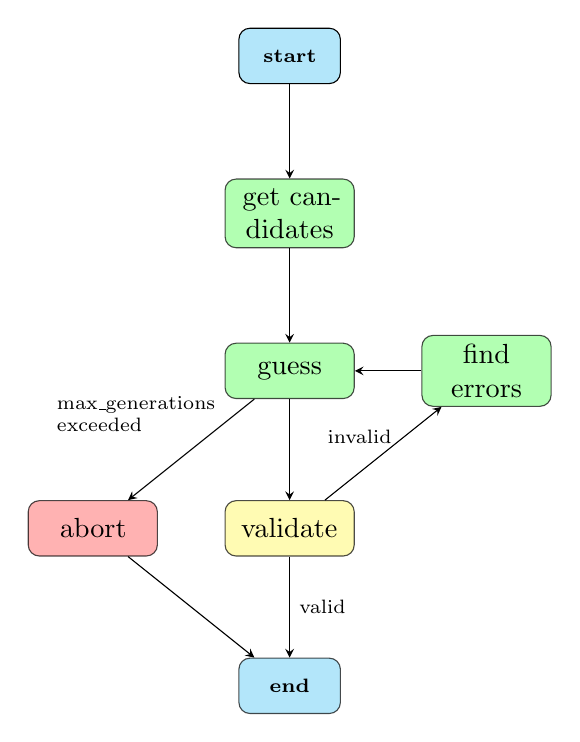
\begin{tikzpicture}[node distance=2cm, align=left]
    
        % nodes
        \node (start) [startend, font=\scriptsize\bfseries] {start};
        \node (get_candidates) [process, below of=start, draw opacity=0.7] {get candidates};
        \node (guess) [process, below of=get_candidates, draw opacity=0.7] {guess};
        \node (validate) [decision, below of=guess, draw opacity=0.7] {validate};
        \node (find_errors) [process, right of=guess, node distance=2.5cm, draw opacity=0.7] {find\\errors};
        \node (abort) [abort, left of=validate, node distance=2.5cm, draw opacity=0.7] {abort};
        \node (end) [startend, below of=validate, font=\scriptsize\bfseries, draw opacity=0.7] {end};
    
        % edges
        \draw [arrow] (start) -- (get_candidates);
        \draw [arrow] (get_candidates) -- (guess);
        \draw [arrow] (guess) -- (validate);
        \draw [arrow] (validate) -- node[midway, right, font=\scriptsize] {valid} (end);
        \draw [arrow] (validate) -- node[midway, above, xshift=-3mm, font=\scriptsize] {invalid} (find_errors);
        \draw [arrow] (find_errors) -- (guess);
        \draw [arrow] (guess) -- node[midway, above, xshift=-7mm, yshift=1mm, font=\scriptsize] {max\_generations\\exceeded} (abort);
        \draw [arrow] (abort) -- (end);
    
    \end{tikzpicture}
    \caption{Workflow of \textit{Llama-itstruct\textsubscript{+cand}}}
    \label{fig:llama-cand}
\end{figure}


Lastly, when suggesting first candidates and referring with those to the tendencies, the LLM relies solely on its own knowledge of the German vocabulary soaked in during the pretraining. That knowledge cannot however provide the model with an absolutely accurate and full access to the vocabulary. For that, in \textit{Llama-instruct\textsubscript{+cand+par}}, I add a tool for looking up words on Wiktionary\footnote{\url{https://de.wiktionary.org/wiki/}}. Beside a large database with German words, an important advantage of Wiktionary is that it also provides genders and morphological paradigms for the entries, which is highly useful since link choice can partially be inferred from the gender, declination type, and the genitive and plural type of the first constituent. The tool is a Python function that sends a GET request to the web server to check the database against the target word, parses the returned HTML fragment for gender and paradigm and heuristically composes a string description of those. Referring to Wiktionary might also be beneficial because if a candidate FC does not exist in the database, it gives a cue that it likely either doesn't exist, or is highly infrequent.

Since the information about the gender and paradigm of the first constituent is used to determine the relevant tendencies, the respective step \textbf{retrieve paradigms} is performed before \textbf{get candidates}. Thus, FC candidates are suggested in \textbf{retrieve paradigms}, morphological info is crawled from Wiktionary for each of them, and they are passed to the next step to be checked against the tendencies; then, the workflow goes the way described for \textit{Llama-instruct\textsubscript{+cand}} (Figure~\ref{fig:llama-par}).


\begin{figure}[hbt!]
    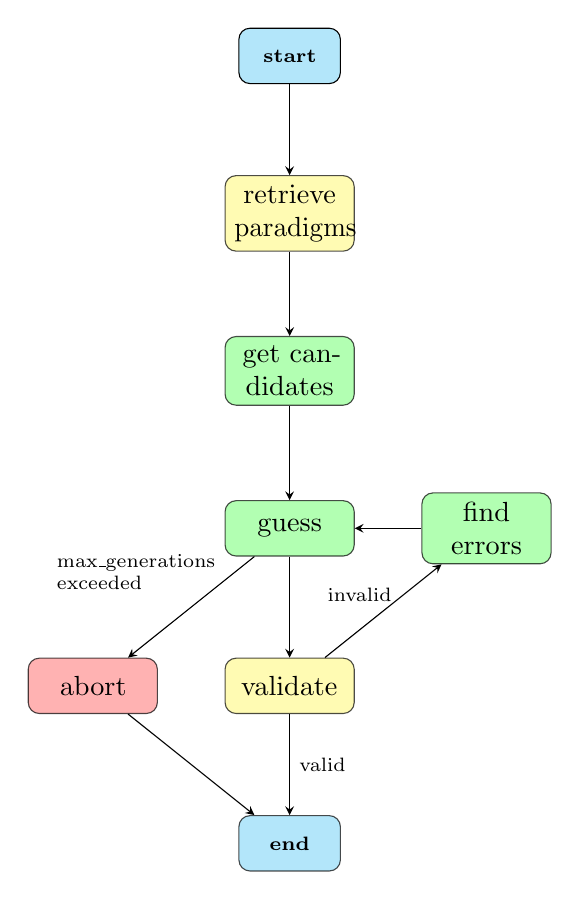
\begin{tikzpicture}[node distance=2cm, align=left]
    
        % nodes
        \node (start) [startend, font=\scriptsize\bfseries] {start};
        \node (retrieve_paradigms) [decision, below of=start, draw opacity=0.7] {retrieve paradigms};
        \node (get_candidates) [process, below of=retrieve_paradigms, draw opacity=0.7] {get candidates};
        \node (guess) [process, below of=get_candidates, draw opacity=0.7] {guess};
        \node (validate) [decision, below of=guess, draw opacity=0.7] {validate};
        \node (find_errors) [process, right of=guess, node distance=2.5cm, draw opacity=0.7] {find\\errors};
        \node (abort) [abort, left of=validate, node distance=2.5cm, draw opacity=0.7] {abort};
        \node (end) [startend, below of=validate, font=\scriptsize\bfseries, draw opacity=0.7] {end};
    
        % edges
        \draw [arrow] (start) -- (retrieve_paradigms);
        \draw [arrow] (retrieve_paradigms) -- (get_candidates);
        \draw [arrow] (get_candidates) -- (guess);
        \draw [arrow] (guess) -- (validate);
        \draw [arrow] (validate) -- node[midway, right, font=\scriptsize] {valid} (end);
        \draw [arrow] (validate) -- node[midway, above, xshift=-3mm, font=\scriptsize] {invalid} (find_errors);
        \draw [arrow] (find_errors) -- (guess);
        \draw [arrow] (guess) -- node[midway, above, xshift=-7mm, yshift=1mm, font=\scriptsize] {max\_generations\\exceeded} (abort);
        \draw [arrow] (abort) -- (end);
    
    \end{tikzpicture}
    \caption{Workflow of \textit{Llama-itstruct\textsubscript{+cand+par}}}
    \label{fig:llama-par}
\end{figure}


To summarize, the LLM-based pipelines implement a CoT with self-reflection, evaluation of own generations, and regeneration as required; throughout the workflow, the LLM reasons decision for the steps, and thus the pipeline navigates the LLM to perform steps depending on the current state. On the first step, the LLM generates a guess with a suggestion of compound analysis. Before this step, a separate LLM can optionally provide possible first constituent and link candidate pairs with reference to the tendencies of link choice, ranked by their probability; for that, another LLM can call a tool to retrieve the genders and paradigms of the suggested FCs. After the guess, the suggested predicted analysis in validated, and if the validation is not passed, a critic LLM with no access to the previous conversation finds the errors in the analysis and forms an instruction for correction. The instruction is given back to the guesser, and a new guess with respect to the pointed errors is made; the regeneration cycle runs until a valid suggestion is made (which stops the generation and outputs the prediction) or \texttt{max\_generations} number is reached (in which case the workflow is aborted and the lemma is returned with no analysis). This implementation of the LLM-based pipelines allows them to self-reflect on their generation and develop the analysis until it is satisfying to be accepted, which should improve the performance of the pipelines on harder compound classes. An example conversation from \textit{Llama-instruct\textsubscript{+cand+par}} is given in Figure~\ref{chat:radiohalter}.


\begin{center}
    \begin{tcolorbox}[colback=gray!10, colframe=black, width=\linewidth, left=1mm, right=1mm, title=Prediction of \texttt{radio\_halter} from \textit{Llama-instruct\textsubscript{+cand+par}}, breakable] %, float=h]
    
        \begin{humanmessage}
            You were given the compound "Radiohalter". Make guesses about which words could be considered to be its first constituent. You have to consider all possible variants. For \textbf{all} these words, you have to look up their paradigms. You have the following tools for this: \\
            
            \textit{<Python function schema>} \\
            
            Form tool calls for \textbf{every} constituent you are considering. As output, give a simple JSON string without additional text containing a list of tool calls. \textit{<more format instructions>}
        \end{humanmessage}

        \begin{toolmessage}{\textbf{retrieve paradigms}}
            There is the word "Radio": a neuter with s-genitive and s plural without umlaut: "des Radios", "die Radios". \\
            There is the word "Halter": a masculine with s-genitive and null plural without umlaut: "des Halters", "die Halter". \\
            The nominative word "Radiohalter" wasn't found and probably doesn't exist.
        \end{toolmessage}

        \begin{humanmessage}
            In German compounds, the properties of the \textbf{first} constituent play a decisive role in choosing the linking element. This means that the \textbf{first} constituent limits the possible choices so that the link can be predicted with some confidence from that. \\
            nThis is described by the following tendencies: \\
            
            \textit{<tendencies from \nameref{sec:appendix:a}>} \\
            
            Your colleague analyzes the compound "Radiohalter". Your task is to define the most probable first constituents and respective linking elements and to sort them by probability with reasoning for that. When choosing, prefer more frequent words. The first constituent should always be nominative. \\
            Always necessary check for the options you suggest to align with the composition of the compound, so that when concatenated the suggested first constituent and linking element, there are no missing or extra elements. \\
            
            \textit{<example>} \\

            Your actual task \\
            ===== \\
            Compound: "Radiohalter" \\
            Hint:
        \end{humanmessage}
        
        \begin{aimessage}{\textbf{get candidates}}
            Based on the provided information, here are the most probable first constituents and respective linking elements for the compound "Radiohalter", sorted by probability with reasoning: \\
            
            1. The first constituent is "Radio". That's a neuter with s-genitive, which points to addition "s". This is the most probable analysis because the word "Radio" is a common and frequent word, and the analysis aligns with the composition of the word. \\
            2. There is no other probable analysis, as no other word with nominative "Radio-" was found. \\
            
            Note that the word "Radiohalter" is not a known compound word, but based on the rules provided, the most likely analysis is that the first constituent is "Radio" with an addition "s" as the linking element. \\
        \end{aimessage}

        \begin{humanmessage}
            You are given a German compound. That is a N+N compound which means it consists of exactly 2 noun constituents with a link in between. There are 4 link types you might encounter: \textit{<list of links with examples>} \\
            
            Your task is to analyze the compound "Radiohalter" in such a way that you define the original constituents and the link as well as the link type from the list above. \\
            
            Your colleague has prepared the most likely pairs of first components and linking elements for you. When choosing, remember that probability is not always correlated with correctness, so be sure to necessarily check which analyses really fit. The hint from the colleague is: \\
            
            \textit{<the output from \textbf{get candidates}>} \\
            

            The output should be a well-formatted JSON instance that strictly conforms to the JSON schema below: \\
            \textit{<JSON schema and format instructions>} \\


            \textit{<here examples can be added dinamically; empty as performing zero-shot>} \\
            
            Your actual task \\
            ===== \\
            Compound: "Radiohalter" \\
            Analysis: \\
        \end{humanmessage}
        
        \begin{aimessage}{\textbf{guess}}
            \begin{verbatim}
{
    "first_noun": "Radio",
    "second_noun": "Halter",
    "link_realization": "s",
    "link_type": "Simple addition"
}
            \end{verbatim}
        \end{aimessage}
    
        \begin{toolmessage}{\textbf{validate}}
            False.
        \end{toolmessage}
    
        \begin{humanmessage}
            Your colleague had the following task: \textit{<initial instructions>}. \\
            This analysis contains error(s) with respect to the task instructions. Find the error(s) and give a one-sentence summary what is wrong in this analysis so that your colleague corrects it. For that, take a careful look at which links may and may not occur in which positions according to the task instructions.
        \end{humanmessage}
    
        \begin{aimessage}{\textbf{find errors}}
            The error in the analysis is that the link realization 's' is not a valid option for "Simple addition" in this position, as according to the task instructions, an -s- link is not specified as a possible link between the constituents when the first noun ends with a vowel, as is the case with "Radio".
        \end{aimessage}
    
        \begin{aimessage}{\textbf{guess}}
            \begin{verbatim}
{
    "first_noun": "Radio",
    "second_noun": "Halter",
    "link_realization": "",
    "link_type": "Concatenation"
}
            \end{verbatim}`
        \end{aimessage}
        
    \end{tcolorbox}
\end{center}
\captionof{figure}{Prediction of \texttt{radio\_halter} from \textit{Llama-instruct\textsubscript{+cand+par}} utilizing all possible steps. Irrelevant parts are omitted}\label{chat:radiohalter}


\subsubsection{Orchestration}

I implement the LLM-based pipelines with \textit{LangChain} and \textit{LangGraph}\footnote{\url{https://python.langchain.com/docs/introduction/} and \url{https://langchain-ai.github.io/langgraph/}, respectively}. LangChain is a framework designed for building LLM-based applications and orchestration of complex workflows involving LLMs. It provides convenient tools for LLM inference, RAG, structured output, defining tools, and much more. LangChain uses Unix-like component piping (LCEL) so that the output of one component becomes the input of the next component; that allows to create complex and fully controlled custom applications with LLMs. LangGraph is designed for easy creation of agentic systems in a graph-like architecture; it is a part of the LangChain ecosystem which makes it compatible with LangChain components and provides easy integration of those. LangGraph operates in terms of nodes and edges, where nodes are steps that might both involve or not involve LLMs, and transitions between steps; conditional transitions allow to define the next step depending on the output of the previous step.

Input compounds are predicted in an asynchronous loop for time efficiency so that while an output of the model for one lemma is waited, the next lemma is being processed; the maximum number of concurrent queries to the Llama3.1 via NVIDIA API is 10. The implementation of the LLM-based pipelines is available under \url{https://github.com/maxschmaltz/DEKOR/blob/main/dekor/splitters/llms/llama_instruct/llama_instruct.py}.


\section{Evaluation}
\label{sec:eval}

\subsection{Metric Overview}

The specificity of the task lays a few constrains of the choice of metrics. Since both the predicted link and the position that it was predicted at matter, the task stands somewhere in between the seq2seq generation and classification tasks (no wonder that the implemented splitters solve one of those); however, none of the classic metrics used for either of these tasks seem to be satisfying. The metrics used for evaluation of the alignment of two sequences (BLEU, METEOR etc.) do not fit our case because, as opposed to the usual seq2seq tasks, even a slight misalignment of tokens is critical (e.g. \texttt{zeit\_erfassung} vs \texttt{zeit\_+er\_fassung}). The usual set of metrics for multi-label classification (precision, recall, F1-score) also does not fit as in compound splitting, not just the link but also the predicted position matters. If the correct link is predicted but on a wrong position, it should be marked as incorrect even though from the purely classificational point of view, it is correct: thus, such metrics can be adjusted for the task, but they will not be transparent enough and will confuse the researchers.

Eventually, it is crucial that both the correct link and the correct position are determined by the models. The metric that can transparently reflect the performance of that models with respect to that is binary accuracy; the analysis is either correct, or it is not. However, accuracy has a disadvantage that has to be handled: it is not adopted for highly imbalanced data. For example, if a model predicts only concatenation correctly, it will still achieve an accuracy score of about 0.6 since there are roughly 60\% of concatenation links in the datasets. Such behavior is undesirable because the models that in fact perform poorly can receive high scores. For that, I gather accuracies across different links separately and weight the scores inversely proportional to their log counts in the test dataset; thus, averaging becomes highly sensitive to underrepresented links and penalizes splitters severely for incorrect predictions of those. The formula of averaging holds:

$$
m_{wa} = \sum_{l \in{L}}{m_l * w_l}
$$

$$
w_l = \frac{1}{log(n_l + 1)} / N
$$

$$
N = \sum_{l \in L} \frac{1}{\log(n_l + 1)}
$$

where $m_{wa}$ is the weighted average of values of a metric, $L$ is the set of links, $m_l$ is the value of the metrics for the link $l$, $w_l$ is its weight; $n_l$ is the count of the link $l$ in the dataset (or a part of it), $W$ is the total log count of all the entries in the dataset (or a part of it); $+1$ is added for Laplace smoothing, $log(n_l + 1)$ is divided by $N$ for scaling to a range $[0, 1]$.


All in all, for each splitter, I provide a table with all predictions, a confusion matrix, a table accuracy for each link as well as the weighted average over all links, and an absolute (normal) accuracy; all listed artifacts are additionally created for each compound class separately\footnote{I will provide only the most insightful and informative table fragments here. The whole collection of results is available under \url{https://github.com/maxschmaltz/DEKOR/tree/main/benchmarking/results/} as well as the respective figures and tables under \url{https://github.com/maxschmaltz/DEKOR/tree/main/benchmarking/figures/}.}.

It is crucial to understand that, since the weighted averaging is highly sensitive to infrequent links and the size of the compound classes, the weighted accuracy scores should be analyzed together with those of the absolute accuracy to give an actual understanding of the models' performance; for example, a low weighted accuracy score with a high absolute accuracy indicates that the model is good at predicting frequent links but tends to fail on more infrequent ones.


\subsection{Average Scores}

\textit{Llama-instruct\textsubscript{+cand+par}} is the best model by the weighted accuracy, a score of 0.677; the model with the best absolute accuracy is \textit{Llama-instruct\textsubscript{base}} achieving a score of 0.861 (see Table~\ref{tab:avg_scores}\footnote{Parameters of the models that the scores are given for can be found in Appendix \nameref{sec:appendix:b}.}). 


\begin{table}[htb!]
    \centering
    \begin{tabular}{@{}lcc@{}}
        \toprule
        Model & Weighted & Absolute \\ \midrule
        \textit{N-gram} & 0.375 & 0.628 \\ \cmidrule{1-3}
        \textit{FFN} & 0.0 & 0.003 \\
        \textit{RNN} & 0.004 & 0.041 \\
        \textit{GRU} & 0.0 & 0.0 \\
        \textit{CNN} & 0.02 & 0.008 \\ \cmidrule{1-3}
        \textit{GBERT} & 0.136 & 0.552 \\
        \textit{ByT5} & 0.4 & 0.721 \\ \midrule
        \textit{Llama-instruct\textsubscript{base}}  & 0.572 & \textbf{0.861} \\
        \textit{Llama-instruct\textsubscript{+cand}} & 0.605 & 0.836 \\
        \textit{Llama-instruct\textsubscript{+cand+par}} & \textbf{0.677} & 0.848 \\ 
        \bottomrule
    \end{tabular}
    \caption{Weighted and absolute accuracy scores of the splitters on average (rounded to 3 digits after decimal point)}
    \label{tab:avg_scores}
\end{table}


This preliminary analysis gives us several preliminary insights on the performance of the models, their weak and strong sides.

\begin{itemize}
    
    \item The models with the masked classification task except for the N-gram model fail to learn the patterns in the data. It seems that either the contexts do not provide enough information to infer the link from that, or it requires more complex pre-processing and/or feature extraction than I implement.

    \item The LLM-based pipelines outperform all the side models on all the metrics on average.

    \item From all the side models, only the N-gram and ByT5-based splitters are somewhat competitive to the LLM-based pipelines.
    
\end{itemize}

To get a deeper understanding of models' performance and the origins of the scores, I will consider scores on compounds with different compound classes below. As the NN-based and the GBERT-based splitters are unable to produce adequate analyses in most of the cases, I will omit theirs results from now on unless required (the rest of the models will be called performant models).


\subsection{Common Compounds}

\begin{table}[htb!]
    \centering
    \begin{tabular}{@{}lcc@{}}
        \toprule
        Model & Weighted & Absolute \\ \midrule
        \textit{N-gram} & 0.2 & 0.675 \\ \cmidrule{1-3}
        \textit{ByT5} & 0.455 & 0.786 \\ \midrule
        \textit{Llama-instruct\textsubscript{base}}  & 0.761 & \textbf{0.921} \\
        \textit{Llama-instruct\textsubscript{+cand}} & 0.743 & 0.897 \\
        \textit{Llama-instruct\textsubscript{+cand+par}} & \textbf{0.857} & 0.902 \\ 
        \bottomrule
    \end{tabular}
    \caption{Weighted and absolute accuracy scores of the performant splitters on the common compounds (rounded to 3 digits after decimal point)}
    \label{tab:common_scores}
\end{table}

Common compounds are the compounds with first constituents forming 60 or more compounds in GeCoDB\_v5. As discussed in \nameref{sec:fc_stats}, common FCs tend to form compounds that are frequent in DECOW16A (hence, on the web) so conditioning on frequency of first constituents works both for the trainable models and the LLM-based pipelines. As expected, the latter outperform all other models: \textit{Llama-instruct\textsubscript{+cand+par}} achieves a weighted accuracy score of 0.857, and \textit{Llama-instruct\textsubscript{base}} --- an absolute accuracy of 0.921 on the common compounds (Figure~\ref{tab:common_scores}).

The result is not surprising as both common first constituent and compounds must be seen by instruct LLMs many times so instruct LLMs' general knowledge and reasoning allow them to analyze the common cases with high quality.


\subsection{Infrequent Compounds \& Hapax Legomena Compounds}


\begin{table}[htb!]
    \centering
    \renewcommand{\arraystretch}{1.02}
    \begin{tabular}{@{}lcc@{}}
        \toprule
        Model & Weighted & Absolute \\ \midrule
        \textit{N-gram} & \makecell{\textbf{0.645} \\ 0.3} & \makecell{0.754 \\ 0.375} \\ \cmidrule{1-3}
        \textit{ByT5} & \makecell{0.355 \\ 0.193} & \makecell{0.595 \\ 0.406} \\ \midrule
        \textit{Llama-instruct\textsubscript{base}} & \makecell{0.376 \\ 0.21} & \makecell{\textbf{0.817} \\ 0.469} & \\
        \textit{Llama-instruct\textsubscript{+cand}} & \makecell{0.468 \\ 0.294} & \makecell{0.77 \\ \textbf{0.5}} & \\
        \textit{Llama-instruct\textsubscript{+cand+par}} & \makecell{0.467 \\ \textbf{0.31}} & \makecell{0.786 \\ \textbf{0.5}} \\ 
        \bottomrule
    \end{tabular}
    \caption{Weighted and absolute accuracy scores of the performant splitters on the infrequent and the hapax legomena (top and bottom, respectively) compounds (rounded to 3 digits after decimal point)}
    \label{tab:inf_scores}
\end{table}

Infrequent compounds are the compounds with the first constituents belonging to 3 to 12 compounds in GeCoDB\_v5; correspondingly, hapax legomena compounds' FCs are unique in GeCoDB\_v5. By testing on infrequent and compounds hapax legomena compounds, I aimed at the models' ability to predict cases they have either seen rarely, or have not seen at all (hapax legomena compounds were excluded from the train datasets).


\begin{table*}[hbt!]
    \centering
    % \resizebox{\textwidth}{!}{%
    \renewcommand{\arraystretch}{1.02}
    \begin{tabular}{@{}lcccccccccccc@{}}
        \toprule
        & \texttt{\_} & \texttt{\_+=e\_} & \texttt{\_+=er\_} & \texttt{\_+e\_} & \texttt{\_+er\_} & \texttt{\_+n\_} & \texttt{\_+ns\_} & \texttt{\_+s\_} & \texttt{\_-e\_} & err\_link & err\_place & none \\ \midrule
        \texttt{\_} & \cellcolor{lightredbg}\makecell{\textbf{64} \\ 48} & 0 & 0 & 0 & 0 & 0 & 0 & 0 & 0 & \makecell{0 \\ 6} & \makecell{0 \\ 13} & \makecell{4 \\ 1} & \\
        \texttt{\_+=e\_} & 0 & \cellcolor{lightredbg}\makecell{0 \\ \textbf{3}} & 0 & 0 & 0 & 0 & 0 & 0 & 0 & \makecell{2 \\ 0} & 0 & \makecell{1 \\ 0} & \\
        \texttt{\_+=er\_} & 0 & 0 & \cellcolor{lightredbg}\makecell{\textbf{3} \\ 2} & 0 & 0 & 0 & 0 & 0 & 0 & \makecell{0 \\ 1} & 0 & 0 & \\
        \texttt{\_+e\_} & 0 & 0 & 0 & \cellcolor{lightredbg}\makecell{1 \\ \textbf{2}} & 0 & 0 & 0 & 0 & 0 & 1 & 0 & \makecell{1 \\ 0} & \\
        \texttt{\_+er\_} & 0 & 0 & 0 & 0 & \cellcolor{lightredbg}\makecell{0 \\ \textbf{1}} & 0 & 0 & 0 & 0 & \makecell{0 \\ 2} & 0 & \makecell{3 \\ 0} & \\
        \texttt{\_+n\_} & 0 & 0 & 0 & 0 & 0 & \cellcolor{lightredbg}\textbf{10} & 0 & 0 & 0 & \makecell{3 \\ 1} & \makecell{0 \\ 3} & \makecell{1 \\ 0} & \\
        \texttt{\_+ns\_} & 0 & 0 & 0 & 0 & 0 & 0 & \cellcolor{lightredbg}\makecell{0 \\ \textbf{3}} & 0 & 0 & \makecell{3 \\ 0} & 0 & 0 & \\
        \texttt{\_+s\_} & 0 & 0 & 0 & 0 & 0 & 0 & 0 & \cellcolor{lightredbg}\makecell{24 \\ \textbf{26}} & 0 & 0 & 0 & \makecell{2 \\ 0} & \\
        \texttt{\_-e\_} & 0 & 0 & 0 & 0 & 0 & 0 & 0 & 0 & \cellcolor{lightredbg}\makecell{\textbf{1} \\ 0} & \makecell{2 \\ 3} & 0 & 0 & \\
        \bottomrule
    \end{tabular}%
    % }
    \caption{Confusion matrix for \textit{Llama-instruct\textsubscript{base}} vs the N-gram splitter (top and bottom, respectively) on the infrequent compounds. A single number is given if equal for both models. "None" stands when the lemma with no analysis was returned, "err\_link" denotes an incorrectly predicted link, "err\_place" denotes that the correct link was predicted but in a wrong position.}
    \label{tab:inf_confmat}
\end{table*}

Comparison of the models on the infrequent compounds exhibits an interesting picture: the N-gram splitter performs with the best weighted accuracy, and all the LLM-based pipelines produce the best absolute accuracy scores (Table~\ref{tab:inf_scores}). This gives us a cue that, while the LLM-based pipelines predict more cases correctly overall, the N-gram splitter manages to predict more infrequent links correctly which affects the weighed average. This intuition is supported by the confusion matrix of the N-gram splitter vs \textit{Llama-instruct\textsubscript{base}} on the infrequent compounds (see Table~\ref{tab:inf_confmat}): there are only few differences between the prediction quality of the two models and they mostly concern infrequent links: addition with umlaut \textit{\underline{e}}, additions \textit{\underline{e}}, \textit{\underline{er}}, and \textit{\underline{ns}} and \textit{\underline{ens}}; more frequent links are predicted on a comparable level or better by the LLM-based pipeline. I suggest that the explanation to that is in the nature of the models in question: there are not that many infrequent compounds with infrequent links in train and test data so during training, the N-gram model sees most of the FC-link pairs for that class; since the N-gram model just remembers the contexts with links, it can easily predict infrequent cases since it has already consumed most of the respective examples.

And while there is a significant gap between the weighted accuracy scores of the N-gram model and the LLM-based pipelines on the infrequent compounds: 0.645 vs 0.468 --- with more or less comparable absolute accuracy scores of 0.754 vs 0.817, the difference of the the weighted accuracy on the hapax legomena compounds is fairly small: 0.3 vs 0.31 --- with much higher absolute accuracy of the LLM-based pipelines: 0.375 vs 0.5, which leads to the conclusion that on the hapax legomena compounds, the infrequent links are predicted on the same level by the both model, while the LLM-based pipelines predict more links correctly overall. As expected, the N-gram model has no zero-shot ability; since it learns contexts by heart during training, it cannot infer links from contexts it as never seen, hence, never learned.

From the other performant models, the LLM-based pipelines confidently outperform the ByT5 splitter on both the infrequent and the hapax legomena compounds (cf. the respective weighted and absolute accuracy scores of \textit{Llama-instruct\textsubscript{+cand+par}} of 0.467 and 0.786, 0.31 and 0.5 vs those of ByT5 of 0.355 and 0.595, 0.193 and 0.406, respectively).

Overall, the N-gram splitter becomes the best to perform on the infrequent compounds with the LLM-based pipelines being better overall, but worse on the infrequent links; the hapax legomena compounds are however predicted significantly better by the LLM-based compounds, confirming my hypothesis of the importance of the zero-shot abilities.


\subsection{Allomorphic FC \& Invented Compounds}

\begin{table}[htb!]
    \centering
    \renewcommand{\arraystretch}{1.02}
    \begin{tabular}{@{}lcc@{}}
        \toprule
        Model & Weighted & Absolute \\ \midrule
        \textit{N-gram} & \makecell{0.072 \\ 0.085} & \makecell{0.353 \\ 0.191} \\ \cmidrule{1-3}
        \textit{ByT5} & \makecell{0.688 \\ 0.606} & \makecell{0.882 \\ 0.702} \\ \midrule
        \textit{Llama-instruct\textsubscript{base}} & \makecell{0.832 \\ 0.837} & \makecell{0.882 \\ 0.766} & \\
        \textit{Llama-instruct\textsubscript{+cand}} & \makecell{\textbf{0.844} \\ 0.882} & \makecell{\textbf{0.941} \\ 0.723} & \\
        \textit{Llama-instruct\textsubscript{+cand+par}} & \makecell{\textbf{0.844} \\ \textbf{0.891}} & \makecell{\textbf{0.941} \\ \textbf{0.787}} \\ 
        \bottomrule
    \end{tabular}
    \caption{Weighted and absolute accuracy scores of the performant splitters on the allomorphic FC and the invented (top and bottom, respectively) compounds\footnote{2 of invented compounds were pre-processed incorrectly, and their analyses were marked as incorrect for all the splitters.} (rounded to 3 digits after decimal point)}
    \label{tab:allomorphy_scores}
\end{table}

The advantages of reasoning can be seen clearly on the compounds with allomorphic first constituents and on the invented compounds. In \nameref{sec:intro} it is suggested that similar inputs mapped to different outputs will probably confuse simple IO models, so allomorphic FC compounds should be problematic for such models, and invented compounds will probably not be analyzed correctly by trainable models for the same reason why hapax legomena compounds are challenging; the distinction between hapax legomena compounds and invented compounds is relevant only for the LLM-based pipelines since, while they may have seen hapax legomena as they exist somewhere on the web, they cannot have seen invented compounds so for these compounds, the reasoning should become the decisive factor.

Allomorphic FC compounds are the compounds whose first constituents show wide variation of link choice. In the test data, there are 2 FCs that occur with 4 different links (\textit{Mann} and \textit{Kind}), and 3 FCs with 3 different links (\textit{Mensch}, \textit{Schwein}, and \textit{Maus}), resulting in 17 compounds\footnote{\url{https://github.com/maxschmaltz/DEKOR/blob/main/dekor/gecodb_datasets/allomorphic_fc.tsv}}.

The invented compounds are taken from \citet{NeefBorgwaldt+2012+27+56}. These compounds describe chimera images and mostly use words for animal designation as constituents. This class of compounds is additionally challenging as their FCs also exhibit allomorphy: as pointed out in \citet{NeefBorgwaldt+2012+27+56}, the participants of the experiment named chimera images with both determinative and copulative compounds which resulted in allomorphy like \texttt{krokodil\_ente} vs \texttt{krokodil\_+s\_ente}. 3 of 22 FCs in invented compounds attach 3 links, other 19 attach 2 links, which makes a total of 47 invented compounds.\footnote{\url{https://github.com/maxschmaltz/DEKOR/blob/main/dekor/gecodb_datasets/invented.tsv}}


Even though the first constituents of these two compounds classes are highly productive --- different allomorphic FCs form 867 to 3079 compounds in GeCoDB\_v, all except for 3 FCs in invented compounds have a productivity of more than 96 with the maximum of 1874 --- none of the side models --- even the performant ones --- get close to the LLM-based pipelines' performance (Table~\ref{tab:allomorphy_scores}). The fact that these two classes are highly challenging due to their variation / uniqueness outweighs the effect of frequency of the FCs for the side models; and here is where the reasoning ability becomes the decisive factor. While ByT5 predicted only one less allomorphic FC compound and 4 less invented compounds correctly compared to \textit{Llama-instruct\textsubscript{+cand+par}}, it mostly failed to predicted less infrequent links on these compounds correctly which explains the gaps in their weighted accuracy scores (0.688 vs 0.844 on the allomorphic FC compounds, 0.606 vs 0.891 on the invented compounds). In some cases where ByT5 failed to predict an infrequent link, \textit{Llama-instruct\textsubscript{+cand+par}} produced a correct prediction on the second or third generation, so in these cases reasoning and self-evaluation led the pipeline to the correct analysis. See a fragment of corrective prediction for an invented compound in Figure~\ref{chat:schwantrompete} as an example. 

The dependency of the N-gram splitter on the seen contexts makes it fail dramatically on the both classes; even though the FCs are frequent, the N-gram splitter has never seen them with such links / second constituents so cannot give adequate analyses for these cases.


\begin{center}
    \begin{tcolorbox}[colback=gray!10, colframe=black, width=\linewidth, left=1mm, right=1mm, title=Prediction of \texttt{schwan\_trompete} from \textit{Llama-instruct\textsubscript{+cand+par}}, breakable]
    
        \begin{humanmessage}
            \textit{<initial prompt>}
        \end{humanmessage}

        \begin{toolmessage}{\textbf{retrieve paradigms}}
            \textit{<retrieved paradigms>}
        \end{toolmessage}
        
        \begin{aimessage}{\textbf{get candidates}}
            \textit{<candidates>}
        \end{aimessage}
        
        \begin{aimessage}{\textbf{guess}}
            \begin{verbatim}
{
    "first_noun": "Schwan",
    "second_noun": "Trompete",
    "link_realization": "e",
    "link_type": "Addition with umlaut"
}
            \end{verbatim}
        \end{aimessage}
    
        \begin{toolmessage}{\textbf{validate}}
            False.
        \end{toolmessage}
    
        \begin{humanmessage}
            Your colleague had the following task: \textit{<initial instructions>}.
            This analysis contains error(s) with respect to the task instructions. Find the error(s) and give a one-sentence summary what is wrong in this analysis so that your colleague corrects it. For that, take a careful look at which links may and may not occur in which positions according to the task instructions.
        \end{humanmessage}
    
        \begin{aimessage}{\textbf{find errors}}
            The error in the analysis is that the link realization 'e' is incorrectly classified as 'Addition with umlaut' because according to the task instructions, an 'e' link can occur in both 'Simple addition' and 'Addition with umlaut', but in 'Addition with umlaut', it should trigger an umlaut in the first noun, which is not the case here, as 'Schwan' does not change to 'Schw{\"a}n'.
        \end{aimessage}
    
        \begin{aimessage}{\textbf{guess}}
            \begin{verbatim}
{
    "first_noun": "Schwan",
    "second_noun": "Trompete",
    "link_realization": "",
    "link_type": "Concatenation"
}
            \end{verbatim}`
        \end{aimessage}
        
    \end{tcolorbox}
\end{center}
\captionof{figure}{CoT for corrective prediction of \texttt{schwan\_trompete} from \textit{Llama-instruct\textsubscript{+cand+par}}. Irrelevant parts are omitted}\label{chat:schwantrompete}


\subsection{Failures of Prediction}

During prediction, splitters sometimes cannot suggest any valid analysis, which results in a \textit{failure} with non-analyzed lemma returned. In case of models with the masked classification task, failure happens when no link passing the filter is predicted for any of the contexts. The seq2seq ByT5 predicts a single analysis; therefore, in contrary to the masked classification models, there is a single option under consideration. Thus, ByT5 fails if it 1) contains invalid links (the same filter for the side models); 2) contains not 1 link exactly; or 3) does not resemble input lemma (i.e. adds or subtracts characters). The LLM-based pipelines have the same conditions of failure but since they have an ability to regenerate analyses, they fail only when each of up to \texttt{max\_generations} generations falls under the conditions. Lastly, the LLM-based pipelines can rarely fail because of timeout or connection errors (the LLMs are hosted on the web), or parsing errors because of incorrectly formed JSONs.

Table~\ref{tab:failures} shows that more infrequent first constituents consistently cause more failures. For all the performant models except for ByT5, prediction for the common compounds fail less often than for the infrequent compounds, and for the latter --- less often than for the hapax legomena compounds. Failures on the allomorphic FC and the invented compounds are more or less comparable with those on the common and the infrequent compounds, respectively. That is explained by the fact that they both have frequent FCs; the allomorphic FC compounds may occur in the train data with all their links but with other second constituents, and invented compounds are more challenging than those as their second constituents are unique for the FCs, which mitigates the effect of the frequency of the latter.

The LLM-based pipelines show a smooth tendency of producing slightly more failures as the complexity of the pipelines grows; that happens due to more hotspots that can become the catalyst for timeouts and parsing errors in more complicated pipelines architectures.

The NN-based pipelines gave no failures; however, analyzing their confusion matrices\footnote{\url{https://github.com/maxschmaltz/DEKOR/tree/main/benchmarking/results/nns}} points out that they 1) predict links arbitrary; and 2) mostly predict concatenation links which cannot lead to a failure. The N-gram splitter produces the least failures from the performant models, which is logical since it learns contexts by heart; that is supported by the fact that on the most unknown contexts (invented compounds), the N-gram splitter yields its largest failures share.

The distribution of the failures of ByT5 is different from other models. Qualitative analysis of its generations\footnote{\url{https://github.com/maxschmaltz/DEKOR/blob/main/benchmarking/results/llms/byt5/final/hapax_legomena/df.tsv}} shows that for the most of the hapax legomena compounds, it predicts concatenations which cannot fail the prediction, and 5 of the 6 failures are made on compounds with explicit target links; that is the reason ByT5 fails much less on the hapax legomena compounds than on the infrequent compounds, and even slightly less than on the common compounds, where it predicts explicit links more often.


\begin{table*}[htb!]
    \centering
    \begin{tabular}{@{}lcccccc@{}}
        \toprule
        Model & common & infrequent & hapax legomena & allomorphic FC & invented & total \\ \midrule
        \textit{N-gram} & 0.032 & 0.008 & 0.0 & 0.0 & 0.149 & 20 \\ \cmidrule{1-7}
        \textit{FFN} & 0.0 & 0.0 & 0.0 & 0.0 & 0.0 & 0 \\
        \textit{RNN} & 0.0 & 0.0 & 0.0 & 0.0 & 0.0 & 0 \\
        \textit{GRU} & 0.0 & 0.0 & 0.0 & 0.0 & 0.0 & 0 \\
        \textit{CNN} & 0.0 & 0.0 & 0.0 & 0.0 & 0.0 & 0 \\ \cmidrule{1-7}
        \textit{GBERT} & 0.29 & 0.333 & 0.485 & 0.412 & 0.362 & 197 \\
        \textit{ByT5} & 0.196 & 0.38 & 0.182 & 0.118 & 0.149 & 143 \\ \midrule
        \textit{Llama-instruct\textsubscript{base}} & 0.054 & 0.093 & 0.364 & 0.059 & 0.17 & 53 \\
        \textit{Llama-instruct\textsubscript{+cand}} & 0.078 & 0.124 & 0.303 & 0.0 & 0.17 & 63 \\
        \textit{Llama-instruct\textsubscript{+cand+par}} & 0.065 & 0.163 & 0.333 & 0.059 & 0.149 & 64 \\
        \bottomrule
    \end{tabular}
    \caption{Failures of the splitters on compounds of different classes. Classes columns show the percents of failed compounds for respective classes (rounded to 3 digits after decimal point). The total column stands for the total numbers of failures for the splitters}
    \label{tab:failures}
\end{table*}


\subsection{Summary}

The summary of the models' performance is fairly short: on average and for all of the compound classes except for the infrequent compounds, the LLM-pipelines perform the best. They achieve the best weighted and absolute accuracy scores in almost all the cases, which means they are good both on frequent and infrequent compound and link classes. The only class that they do not outperform the other splitters on is the infrequent compounds, where they are the second model standing closely after the N-gram splitter.

From the side models, only the N-gram and the ByT5 splitters are more or less comparable to the LLM-based pipelines. However, the N-gram model relies on remembering context-link masks which determines its low performance on low-frequency compound classes and on compounds it has never seen. That said, the ByT5 splitter is the only side model that consistently produces high quality results for compounds and links of different classes and gets close to the LLM-based pipelines by performance.

Below in section \nameref{sec:disc}, I investigate different factors and their effects on performance of the models.


\section{Discussion}
\label{sec:disc}

\subsection{Compound Class}

\begin{table*}[htb!]
    \centering
    \renewcommand{\arraystretch}{1.02}
    \begin{tabular}{@{}lccccc@{}}
        \toprule
        Model & common & infrequent & hapax legomena & allomorphic FC & invented \\ \midrule
        \textit{N-gram} & \makecell{0.2 \\ 0.675} & \makecell{\textbf{0.645} \\ 0.754} & \makecell{0.3 \\ 0.375} & \makecell{0.072 \\ 0.353} & \makecell{0.085 \\ 0.191} \\ \cmidrule{1-6}
        \textit{FFN} & \makecell{0.0 \\ 0.005} & 0.0 & 0.0 & 0.0 & 0.0 & \\
        \textit{RNN} & \makecell{0.003 \\ 0.049} & \makecell{0.002 \\ 0.024} & \makecell{0.004 \\ 0.031} & 0.0 & \makecell{0.006 \\ 0.043} & \\
        \textit{GRU} & 0.0 & 0.0 & 0.0 & 0.0 & 0.0 & \\
        \textit{CNN} & \makecell{0.001 \\ 0.003} & \makecell{0.003 \\ 0.016} & \makecell{0.004 \\ 0.031} & 0.0 & \makecell{0.264 \\ 0.021} \\ \cmidrule{1-6}
        \textit{GBERT} & \makecell{0.097 \\ 0.626} & \makecell{0.14 \\ 0.508} & \makecell{0.208 \\ 0.281} & \makecell{0.072 \\ 0.353} & \makecell{0.139 \\ 0.34} & \\
        \textit{ByT5} & \makecell{0.455 \\ 0.786} & \makecell{0.355 \\ 0.595} & \makecell{0.193 \\ 0.406} & \makecell{0.688 \\ 0.882} & \makecell{0.606 \\ 0.702} \\ \midrule
        \textit{Llama-instruct\textsubscript{base}} & \makecell{0.761 \\ \textbf{0.921}} & \makecell{0.376 \\ \textbf{0.817}} & \makecell{0.21 \\ 0.469} & \makecell{0.832 \\ 0.882} & \makecell{0.837 \\ 0.766} & \\
        \textit{Llama-instruct\textsubscript{+cand}} & \makecell{0.743 \\ 0.897} & \makecell{0.468 \\ 0.77} & \makecell{0.294 \\ \textbf{0.5}} & \makecell{\textbf{0.844} \\ \textbf{0.941}} & \makecell{0.882 \\ 0.723} & \\
        \textit{Llama-instruct\textsubscript{+cand+par}} & \makecell{\textbf{0.857} \\ 0.902} & \makecell{0.467 \\ 0.786} & \makecell{\textbf{0.31} \\ \textbf{0.5}} & \makecell{\textbf{0.844} \\ \textbf{0.941}} & \makecell{\textbf{0.891} \\ \textbf{0.787}} \\
        \bottomrule
    \end{tabular}
    \caption{Weighted and absolute accuracy scores (top and bottom, respectively) for the splitters against compound classes (rounded to 3 digits after decimal point)}
    \label{tab:metrics_by_classes}
\end{table*}

As anticipated, the productivity of the first constituent severely affects the performance of the splitters, both the side models and the LLM-based pipelines (see Table~\ref{tab:metrics_by_classes}). Weighted and absolute accuracy decrease consistently from the common through the infrequent to the hapax legomena compounds, which tells us that the splitters struggle to detect the link correctly as the frequency of the FC declines. It is not the case only for the N-gram splitter, who benefits from a lesser number of infrequent compounds combined with its ability to remember compound-link pairs from a couple of observations. Since there is a connection between the FC productivity and its compounds frequencies, both the trainable models and the LLM-based pipelines suffer from the lack of observations of the FCs of the infrequent and the hapax legomena compounds; thus, the observed effect if relevant for all the splitters (except for the discussed performance of the N-gram model on infrequent compounds).

The situation is different with the allomorphic FC and invented compounds. For the models that cannot \textbf{train} a persistent ability to predict correct links from common compounds (and the majority of the FCs from these two classes are frequent), these two classes are highly challenging. For instance, the N-gram model that can only remember contexts and not \textbf{train} on them gives the worse performance from all classes for the both considered metrics; the NN-based models' performance is in level with their performance on other classes due to their inability to learn any patterns; for the GBERT-splitter, these two classes take the middle position by performance between the hapax legomena and the infrequent compounds. The other pattern is seen for the models with strong ability to predict common compounds --- the ByT5-based splitter and the LLM-based pipelines. These models exhibit even better performance on these two classes than on the other three, most likely, due to the reduced size of those. When it comes to the allomorphic FC and the invented compounds, not only reasoning and language knowledge, but also the ability to look up information about the candidates becomes the success factor, which is pointed out by the fact, that \textit{Llama-instruct\textsubscript{+cand+par}} is the absolute winner for this compound classes; since the FCs of invented compounds are common but appear with different links / never appear with the given links and second constituents, their analysis is similar to assembling a completely new puzzle from known detail, where tool calling can give some parts of the reference picture.

Thus, I make a conclusion that in general, all splitters --- including the LLM-based pipelines --- show a tendency of better performance on compounds with more frequent first constituents.


\subsection{Link Frequency}

\begin{table*}[htb!]
    \centering
    \renewcommand{\arraystretch}{1.02}
    \begin{tabular}{@{}lccccccccc@{}}
        \toprule
        Model & \texttt{\_} & \texttt{\_+=e\_} & \texttt{\_+=er\_} & \texttt{\_+e\_} & \texttt{\_+er\_} & \texttt{\_+n\_} & \texttt{\_+ns\_} & \texttt{\_+s\_} & \texttt{\_-e\_} \\ \midrule
        
        \textit{N-gram} & 0.624 & \textbf{0.571} & 0.25 & 0.267 & 0.182 & 0.636 & 0.444 & 0.816 & 0.0 \\ \cmidrule{1-10}
        
        \textit{FFN} & 0.006 & 0.0 & 0.0 & 0.0 & 0.0 & 0.0 & 0.0 & 0.0 & 0.0 \\
        
        \textit{RNN} & 0.073 & 0.0 & 0.0 & 0.0 & 0.0 & 0.0 & 0.0 & 0.0 & 0.0 \\
        
        \textit{GRU} & 0.0 & 0.0 & 0.0 & 0.0 & 0.0 & 0.0 & 0.0 & 0.0 & 0.0 \\
        
        \textit{CNN} & 0.006 & 0.0 & 0.125 & 0.0 & 0.0 & 0.0 & 0.0 & 0.016 & 0.0 \\ \cmidrule{1-10}
        
        \textit{GBERT} & 0.489 & 0.0 & 0.0 & 0.0 & 0.0 & 0.649 & 0.0 & 0.928 & 0.0 \\
        
        \textit{ByT5} & 0.893 & 0.0 & 0.0 & \textbf{0.533} & \textbf{0.727} & 0.623 & 0.333 & 0.48 & \textbf{0.583} \\ \midrule
        
        \textit{Llama-instruct\textsubscript{base}} & \textbf{0.905} & 0.429 & \textbf{1.0} & 0.4 & 0.364 & 0.844 & 0.222 & 0.952 & 0.5 \\
        
        \textit{Llama-instruct\textsubscript{+cand}} & 0.835 & 0.286 & 0.5 & \textbf{0.533} & 0.455 & \textbf{0.87} & \textbf{0.889} & \textbf{0.96} & \textbf{0.583} \\
        
        \textit{Llama-instruct\textsubscript{+cand+par}} & 0.862 & 0.429 & \textbf{1.0} & \textbf{0.533} & 0.364 & \textbf{0.87} & \textbf{0.889} & 0.92 & 0.5 \\
        
        \bottomrule
    \end{tabular}
    \caption{Absolute accuracy scores for the splitters against links (rounded to 3 digits after decimal point)}
    \label{tab:metrics_by_links}
\end{table*}


Table~\ref{tab:metrics_by_links} gives a clear picture of dependency of models' performance from link frequency. In section \nameref{subsec:link_distr} it was stated that there are only 5 frequent links in GeCoDB\_v5: concatenation \textit{\underline{ }}, \textit{\underline{s}} and \textit{\underline{es}}, \textit{\underline{n}} and \textit{\underline{en}}; they are parsed as \texttt{\_}, \texttt{\_+s\_}, and \texttt{\_+n\_}, respectively. These 3 links (the 5 become 3 after eliminative parsing) make up 96.82\% of all the links in the corpus. Their frequency determines higher absolutely accuracy scores that the splitters consistently achieve on them; for the most of the models, there can be seen a clear distinction between the frequent and the infrequent links in terms of performance. For instance, the N-gram and the ByT5 splitters show a strong performance on the frequent links but lower scores on the infrequent links, while also failing to predict a few links completely; the GBERT-based splitter predicts exactly the 3 frequent links with weighted and absolute accuracies approximating the performant models while totally failing to detect any infrequent links. The contrast between the two groups is clearly presented by the fact that for all the splitters --- even for the unsucessful NN-based models --- the most frequent link (concatenation) is predicted with the best or close-best scores, while the two most infrequent links (addition with umlaut \textit{\underline{e}} and additions \textit{\underline{ns}} and \textit{\underline{ens}}) achieve the worst metrics for the most of the splitters.

Decrease of the accuracy scores for the infrequent links is noticeably less for the LLM-based pipelines than for the other splitters. While the infrequent links are predicted with lower accuracy, indeed, the differences are not too significant compared to the other models, and the difference is generally reduced as the pipeline becomes more complex. Thus, \textit{Llama-instruct\textsubscript{+cand+par}} does not go beyond an accuracy score of 0.363 for any of the links, and for some infrequent links (addition with umlaut \textit{\underline{er}}, \textit{\underline{ns}} and \textit{\underline{ens}}), it exhibits near-perfect weighted and absolute accuracy; also, the LLM-based pipelines are the only splitters that do not have a zero performance on any of the links.

To summarize, all the splitters --- the LLM-based pipelines included --- perform better on frequent links, often with a significant gap between frequent and infrequent links. For the LLM-based pipelines, this effect may be explained by the tendency of LLMs to perform worse when less probable outputs are expected \cite{mccoy2023embersautoregressionunderstandinglarge}; the very task of Next Word Prediction presets that in case of multiple candidate generations, the most probable token sequence conditioned by the previously generated / input tokens should be preferred, and if Llama3.1 "knows" something about German compounding, it is more likely to be information about or examples of more frequent links.


\subsection{Training Setup and Splitter Task}

From the models with the masked classification tasks, only the N-gram splitter produces adequate results, the other models (all the NN-based and the GBERT-based splitters) do not even reach a weighted accuracy score of 0.14 on average (Table~\ref{tab:avg_scores}). The explanation to that may be that the contexts retrieved for training and prediction do not provide any grammatical information and can only give some phonological and prosodical cues, while grammatical features are much more relevant for link choice than prosodical features. These contexts just do not bear enough information to learn any patterns. See Figure~\ref{fig:losses} that shows the loss plots for the NN-based models; one can clearly see that the training fails as the models do not find how they should adjust their parameters to approximate the distribution. Only the FFN shows a very slight positive trend, but training for a longer time does not change its results significantly: increasing the number of training epochs from 10 to 100 increased the weighted accuracy score only from 0.0 to 0.001\footnote{Excluding the results for concatenation with umlaut.} even though the loss values maintained the trend (this experiment was run separately).

\begin{figure*}[hbt!]
    \centering
    \includegraphics[width=\textwidth]{figs/nn_loss_plots.png}
    \caption{Loss plots for NN-based splitters}
    \label{fig:losses}
\end{figure*}

What concerns train sizes, their impact is random on the NN-based models as it can be anticipated for the models that are not learning patterns from the data; Figure~\ref{fig:train_sizes} shows that there is no trend for dependency of F1-score\footnote{Just like with hyperparameters, evaluation on different training sizes were made on the previous iteration so it used F1-score and includes concatenation with umlaut. Once again, in this case the relative and not the absolute scores are important for drawing conclusions.} from training size that would cover all NN-based models. I suppose this effect is not related to overfitting and only indicate that the training fails.

\begin{figure*}[hbt]
    \centering
    \includegraphics[width=\textwidth]{figs/f1_vs_train_size.png}
    \caption{F1-score vs train sizes for the NN-based models}
    \label{fig:train_sizes}
\end{figure*}


Another reason why the NN-based models might not learn anything can be that their architecture is just too simple to learn such complex patterns from little informative contexts. As it was already mentioned, these models were designed more as drafts of the larger-scale analogues, which might have lead to oversimplification. A hint to that is given by the fact that, even though having the same task, the GBERT-splitter with a much more sophisticated architecture did actually find meaningful signals in the data and it benefit from larger train sizes (Figure~\ref{fig:train_sizes_llms}).

\begin{figure*}[hbt!]
    \centering
    \includegraphics[width=\textwidth]{figs/f1_vs_train_size_llms.png}
    \caption{F1-score vs train sizes for the simple-LLM-based models}
    \label{fig:train_sizes_llms}
\end{figure*}


Lastly, the N-gram model performs much better than the other masked classification models because it does not have to generalize the data and understand patterns; its goal is (simply saying) to learn by heart as many compounds as possible. It is supported by the fact that the most of the model's correct prediction come from the compounds whose first constituents it has seen (common, infrequent FCs) while the weighted accuracy on the compounds with allomorphic FCs (those were excluded from the training datasets) and the invented compounds is under 0.073 and 0.086 respectively (see Table~\ref{tab:allomorphy_scores}).


The seq2seq generation task seems to be much better for the splitters; the ByT5-based splitter achieves high results in all the compound classes and is almost competitive to the LLM-based pipelines. The reason may lie in the fact that such models are originally designed for attention-based mapping from the tokens in the input sequence to the tokens from the output sequence. That "attentive" mapping gives ByT5 much more "understanding" which parts of input sequence should remain untouched, and where a link must be inserted; seq2seq models are more flexible, they see the whole picture and can build complex non-linear mappings (cf. machine translation for languages with different word order). In case of ByT5, it is also a character-level model which, in addition to its seq2seq task, allows it to define quite accurately which character sequences entail which links.

Lastly, instruct text generation joins the advantages of seq2seq models with much larger general knowledge and the ability for reasoning. The first allows instruct LLMs be used on non-trivial tasks without fine-tuning; cf. scores of ByT5 vs the LLM-based pipelines, while ByT5 required almost 50k of train examples and the LLM-based pipelines were performing zero-shot generation without additional fine-tuning. Moreover, the reasoning abilities allow the LLM-based pipelines to outperform the seq2seq ByT5-based splitter not only on common compounds but also on all challenging cases: the infrequent compounds and the hapax legomena compounds are predicted by different LLM-based pipelines with almost equal to significantly better weighted and in all cases much higher absolute accuracy (Table~\ref{tab:inf_scores}); the allomorphic FC compounds and the invented compounds are predicted by the LLM-based pipelines with comparable absolute accuracy scores and a significant gap in weighted accuracy (Table~\ref{tab:allomorphy_scores}).


\subsection{Configuration of the LLM-based Pipelines}

\subsubsection{Hyperparameters}

Here, I consider the impact of the language and the number $n$ of shots on performance of the pipeline. Similarly to hyperparameters etc. for trainable models, I first ran evaluation on test-100\footnote{As opposed to hyperparameter tuning for the side models, I exclude the results for concatenation with umlaut for the LLM-based pipelines.} with \texttt{max\_generations=2} to define the best configuration for further analysis.

All the prompts are available both on English and German. The intuition was, since Llama3.1 is multilingual and understands German, it might benefit from German instructions because 1) there might have been literature from the relevant scientific domain in German in its training data; 2) it wouldn't have to switch languages during generation. However, it turned out to be not the case. On the English instructions, \textit{Llama-instruct\textsubscript{base}} outperforms its German variant with a significant gap in both weighted and absolute accuracy (Figure~\ref{tab:hyperparams_llama}). There is a simple explanation to this phenomenon: even though Llama3.1 understands German, most of its data contains "significantly more English tokens than non-English tokens" \cite{dubey2024llama3herdmodels}; although extensive post-training on multilingual data was conducted after pretraining, English remains Llama3.1's "primary language". Qualitative analysis shows that the German version sometimes gets confused on character level and cannot define constituent borders; most often, that leads to the situation when it assigns the same span both to a constituent and the link if the beginning of the first or the end of the second constituent. For example, it predicts that \texttt{k{\"u}lte\_schrank} has a link \texttt{\_+s\_} between \texttt{k{\"u}lte} and \texttt{schrank} (attributes the segment \textit{-s-} both to the link and the second constituent); the same example is found in invented \texttt{alligator\_ente}, where the splitter predicts a link \texttt{\_+en\_} before the second constituent \texttt{ente}; in such cases, the German version of the LLM on the \textbf{find error} step also does not determine the mistake.

The number of shots also gives the opposite effect from what one would expect; usually, $n$-shot prompting slightly increases performance of an LLM (e.g. \citealt{brown2020languagemodelsfewshotlearners}), but not with the LLM-based pipelines. With them, zero-shot prediction appears to produce better analyses compared to 3-shot prompting (Figure~\ref{tab:hyperparams_llama}). I don't find any particular reason for that after analyzing the generations of the model for the same inputs with zero-\footnote{\url{https://github.com/maxschmaltz/DEKOR/blob/main/benchmarking/results/llms/llama-instruct/hyperparameters/base_english_0_shot_small/messages.json}} and 3-shot\footnote{\url{https://github.com/maxschmaltz/DEKOR/blob/main/benchmarking/results/llms/llama-instruct/hyperparameters/base_english_3_shot_small/messages.json}} prompting.

\begin{table}[htb!]
    \centering
    \renewcommand{\arraystretch}{1.02}
    \begin{tabular}{@{}lcc@{}}
        \toprule
         & zero-shot & 3-shot \\ \midrule
        English & \scalebox{1}{\makecell{\textbf{0.646} \\ \textbf{0.784}}} & \scalebox{1}{\makecell{0.582 \\ 0.769}} \\ %\cmidrule{1-3}
        German & --- & \scalebox{1}{\makecell{0.5 \\ 0.697}} \\
        \bottomrule
    \end{tabular}
    \caption{Weighted and absolute accuracy scores (top and bottom, respectively) of different configurations of \textit{Llama-instruct\textsubscript{base}} on test-100 (rounded to 3 digits after decimal point)}
    \label{tab:hyperparams_llama}
\end{table}


For evaluation on test-500, I used the best parameters obtained from hyperparameter evaluation, namely, I run the LLM-based pipelines on the zero-shot English prompts.


\subsubsection{Pipeline Components}

\textit{Llama-instruct\textsubscript{+cand}} and \textit{Llama-instruct\textsubscript{+cand+par}} consistently become the best of the LLM-pipelines (target metric: weighted accuracy); \textit{Llama-instruct\textsubscript{+cand}} becomes better on infrequent compounds (Table~\ref{tab:inf_scores}), and \textit{Llama-instruct\textsubscript{+cand+par}} --- on all other classes as well as on average (Tables \ref{tab:common_scores}, \ref{tab:inf_scores}, \ref{tab:allomorphy_scores}, \ref{tab:avg_scores}).

Comparison of the generations of \textit{Llama-instruct\textsubscript{base}}\footnote{\url{https://github.com/maxschmaltz/DEKOR/blob/main/benchmarking/results/llms/llama-instruct/cand_english_0_shot/df.tsv}} and \textit{Llama-instruct\textsubscript{+cand}}\footnote{\url{https://github.com/maxschmaltz/DEKOR/blob/main/benchmarking/results/llms/llama-instruct/base_english_0_shot/df.tsv}} reveals that consistently, the LLM cannot generate correct analyses without candidates and a reference to tendencies of German compounding; in such cases, \textit{Llama-instruct\textsubscript{base}} generates arbitrary incorrect analyses until \texttt{max\_generations} is reached, and \textit{Llama-instruct\textsubscript{+cand}} suggest candidates that guide the LLM to correct generations (cf. generations of the two pipelines on compounds \texttt{beweis\_element}, \texttt{zivildienst\_erfahrung}, \texttt{bediener\_eingriff}, \texttt{haus\_hoheit}, links to the files with the generations are provided in the footnote); interestingly, \textit{Llama-instruct\textsubscript{+cand}} does not always suggest candidates with the correct one among them, but it still helps the LLM to produce a correct analysis after all. The benefits of candidate suggestion is mostly noticed on common compounds; if an infrequent or a hapax legomena compound fails with \textit{Llama-instruct\textsubscript{base}}, it most often often fails with \textit{Llama-instruct\textsubscript{+cand}} as well (cf. \texttt{sch{\"u}ppe\_+n\_stra{\ss}e}, \texttt{staend\_+e\_staat}).

Due to the ability of \textit{Llama-instruct\textsubscript{+cand+par}} to refer to a large database of German words --- Wiktionary --- to retrieve genders and paradigms of the candidate first constituents (if they are present in this database), it lets the LLM on the \textbf{get candidates} step pick relevant tendencies more precisely and, hence, produce more accurate candidates. Furthermore, the absence of a word on Wiktionary gives a strong cue to its non-existence or very low frequency, which naturally filters out improbable candidates. Compare the difference of generated candidates of \textit{Llama-instruct\textsubscript{+cand}} and \textit{Llama-instruct\textsubscript{+cand+par}} for compound \texttt{meer\_land} in Figures \ref{chat:meerland_cand} and \ref{chat:meerland_cand_par}, respectively. There, \textit{Llama-instruct\textsubscript{+cand}} makes inference to the tendencies but takes a tendency that matches ("addition 'es' or 's'") and applies it without further consideration (1), while also producing impossible candidates (2-4); that makes the \textbf{get candidates} LLM mark an incorrect analysis as the most probable. \textit{Llama-instruct\textsubscript{+cand+par}}, on contrary, explicitly lays off all other analysis and states the only probable candidate, which appears to be the correct answer.

\begin{center}
    \begin{tcolorbox}[colback=gray!10, colframe=black, width=\linewidth, left=1mm, right=1mm, title=Candidates for \texttt{meer\_land} from \textit{Llama-instruct\textsubscript{+cand+par}}]
        
        \begin{aimessage}{\textbf{get candidates}}
            Based on the provided information, here are the possible analyses for the compound "Meerland":
            
            1. The first constituent is "Meer". As a neuter with s-genitive, it points to addition "s". However, since the compound is "Meerland" and not "Meersland", this analysis is not possible.
            
            2. The first constituent is "Meer" with concatenation. This is the most probable analysis, as "Meer" is a frequent word and concatenation is the default for German compounds when the first constituent is not from any of the above classes.
            
            There are no other possible analyses, as the words "Mee", "Meerl", and "Meerland" do not exist as nominative words.
            
            Therefore, the most probable analysis is: 1. The first constituent is "Meer" with concatenation.
        \end{aimessage}
        
        
    \end{tcolorbox}
\end{center}
\captionof{figure}{Candidates for \texttt{meer\_land} from \textit{Llama-instruct\textsubscript{+cand+par}}}\label{chat:meerland_cand_par}


\begin{center}
    \begin{tcolorbox}[colback=gray!10, colframe=black, width=\linewidth, left=1mm, right=1mm, title=Candidates for \texttt{meer\_land} from \textit{Llama-instruct\textsubscript{+cand}}]
        
        \begin{aimessage}{\textbf{get candidates}}
            Based on the provided rules and tendencies, I'll analyze the compound "Meerland" and suggest the most probable first constituents and respective linking elements, sorted by probability with reasoning.
            
            1. The first constituent is "Meer". This is a strong neuter noun with (e)s-genitive, which points to addition "es" or "s". However, since "Meer" ends with a consonant and not a suffix that typically takes "s" as a linking element, I'll opt for addition "es" as the more probable choice. This analysis aligns with the composition of the word, and "Meer" is a relatively frequent word.
            Probability: High
            
            2. The first constituent is "Meere", which would point to addition "s". However, this analysis is less probable because "Meere" is not as frequent as "Meer", and the addition "s" is not as common with neuter nouns.
            Probability: Medium
            
            3. The first constituent is "Meerland" itself, with no linking element (concatenation). This analysis is possible, but less probable, as "Meerland" is not a copulative compound, and concatenation is not the default for neuter nouns.
            Probability: Low
            
            4. The first constituent is "Meeres", which would imply concatenation, as the linking element "es" is already included in the first constituent. However, this analysis is the most improbable, as there is no such word with nominative "Meeres".
            Probability: Very Low
            
            In conclusion, the most probable analysis is that the first constituent is "Meer" with addition "es" as the linking element.
        \end{aimessage}        
        
    \end{tcolorbox}
\end{center}
\captionof{figure}{Candidates for \texttt{meer\_land} from \textit{Llama-instruct\textsubscript{+cand}}}\label{chat:meerland_cand}


\textit{Llama-instruct\textsubscript{+cand+par}}'s access to external information in real time lets it suggest cleaner and less hallucinatory candidate generations, which naturally improves the performance of the pipeline. In general, the tendency is seen on the LLM-based pipelines that the more access to quality verified information it has (tendencies, paradigms), the more signals it can receive from the outer world that guide it in the right direction; higher performance is a consequence of receiving such signals. 

The ability of the LLM-based pipelines to evaluate own generations and build CoTs on how to regenerate the result correctly is also highly impactful. Thanks to the \textbf{guess}---\textbf{validate}---\textbf{find errors}---\textbf{guess} cycle, many incorrect otherwise generations are refined; most importantly, the LLM-based pipelines are able to \textbf{reason} why certain analyses are incorrect and then guide themselves to the correct prediction based on this reasoning (examples are given in Figures \ref{chat:radiohalter}, \ref{chat:schwantrompete}). From 591 compounds in test-500, for each LLM-based pipelines, more than 24 compounds are predicted correctly after the first regeneration and up to 30 --- after the second regeneration (Table~\ref{tab:regenerations}). This is an evidence that self-evaluation and critical reasoning abilities combined with the ability to regenerate the answer after taking into account this reasoning can significantly improve LLM's outputs, including for compound splitting.


\begin{table}[htb!]
    \centering
    \renewcommand{\arraystretch}{1.02}
    \begin{tabular}{@{}lcc@{}}
        \toprule
         & 1 & 2 \\ \midrule
         \textit{Llama-instruct\textsubscript{base}} & 24 & 3 \\
         \textit{Llama-instruct\textsubscript{+cand}} & 87 & 9 \\
         \textit{Llama-instruct\textsubscript{+cand+par}} & 95 & 30 \\
        \bottomrule
    \end{tabular}
    \caption{Numbers of compounds, predicted correctly after $k$ regenerations on test-500 (from 591 compounds)}
    \label{tab:regenerations}
\end{table}


\subsection{Dataset Noise}

Lastly, rare prediction errors were caused by the noise in the dataset.

First, there are several occurrences in the test data in which umlauts are written as diphtongs (cf. \texttt{staend\_+e\_staat} for \textit{St{\"a}nd\underline{e}staat}). Such compounds cannot be predicted correctly with the LLM based pipelines because they are fine-tuned to ignore human typos and thus replace the diphtongic spelling with the respective single character; for example, \textit{Llama-instruct\textsubscript{base}} gives a correct prediction which is however not accepted because of that:

\begin{verbatim}
{
    "first_noun": "Stand"
    "second_noun": "Staat",
    "link_realization": "e",
    "link_type": "Addition with umlaut"
}
\end{verbatim}

Second, some misanalyses from SMOR that got to the test data as gold analyses, lead to declined correct analyses. For instance, in \textit{Fach\underline{ }simplerei}, the affix \textit{-ei} was misanalyzed as the second constituent \textit{Ei 'egg'} which results in an erroneous record in the data: \texttt{fachsimpler\_ei}; due to that, the correct prediction \texttt{fach\_simplerei} from {Llama-instruct\textsubscript{+cand}} is rejected.

Those are the examples of noise that do not affect evaluation severely; there are merely a couple of such cases in the whole test data. This noise should however be kept in mind to avoid its inference in later iterations of the research.


\section{Conclusion}
\label{sec:conclusion}

The productivity of compounding in German poses a problem for natural language processing on German material, since it limitlessly inflates its vocabulary. One of the ways to handle this issue is to build a compound splitter. There are two main challenges when it comes to compound splitting: 1) German has a large inventory of linking elements whose frequency is largely scattered, which highly complicates finding constituent boundaries; choice of linking elements does not follow any certain rules and cannot be deterministically inferred from any features of compounds; 2) the high productivity of compounding leads to an extremely uneven distribution of compound frequencies, where the most of the compounds are very infrequent or even unique; furthermore, new compounds may be spontaneously created with little to no limitations. While there are different approaches producing high performance, they are either bound to a certain lexicon, or ignore (most of) the links. In this thesis, I present LLM-based pipelines for compound splitting that are designed to handle N+N compounds of any frequency with 12 different links. The pipelines use self-evaluation and self-critique to regenerate analyses if needed and are capable of reasoning their decisions in a form of chain of thoughts that guides them to correct analysis; different LLM-pipelines have different levels of access to external information. 

The pipelines consistently outperform the other compared splitters on all compound classes except for infrequent compounds where they perform second-best; out of 12 links, the pipelines achieve a near-perfect performance on the 5 most frequent links and perform with an adequate quality on infrequent links. The best LLM-pipeline \textit{Llama-instruct\textsubscript{+cand+par}} generates possible first constituents, looks up their genders and paradigms on Wiktionary, compares the gathered info against the tendencies of German compounding, ranks possible candidates and then makes a guess about compound analysis. It performs the best on average and achieves a weighted accuracy score of 0.677 and an absolute accuracy of 0.848 over 591 test compounds. Its generations give evidence that a chain of thoughts manner of generations combined with the abilities to evaluate own generations for possible regeneration and to access validated information from outside of the model increase the performance of the LLM-based pipelines on the task of compound splitting significantly.

Another important conclusion from this research is the fact that instruct LLMs are potentially capable of solving non-trivial and complex \textbf{linguistic} tasks. On the example of compound splitting it was shown, that such LLMs can be combined with other artifacts and tools to compile complex pipelines with conditional routing, self-evaluation, and decision-making. While not achieving the perfect performance, such pipelines might be the first step to building smart LLM-based systems to conduct complex linguistic analysis and research.


\bibliography{custom}
\bibliographystyle{acl_natbib}
% \bibliographystyle{plainnat}

\appendix
\section{Tendencies of German Compounding}
\label{sec:appendix:a}

The following document serves as the instructions for the LLM-based pipelines that describe the tendencies of link choice from grammatical (and sometimes semantic and prosodic) properties of the first constituent:

{
    % disable section numbering in context mode to prevent MD headers to be read as subsections
    \setcounter{secnumdepth}{0}
    \small
    \markdownInput{cat_tendencies_english.md}
    \setcounter{secnumdepth}{3}  % back to default
}


\section{Parameters of Splitters}
\label{sec:appendix:b}

Parameters and train sizes of the models for final evaluation are given below.

\begin{itemize}
    
    \item \textit{N-gram} (train-50k): \\ \\
    \texttt{n=2} \quad maximum N-grams length \\
    \texttt{record\_none\_links=False} \quad whether to record contexts between which no links occur \\

    \item \textit{FFN} (train-10k): \\ \\
    \texttt{context\_window=2} \quad maximum N-grams length \\
    \texttt{record\_none\_links=False} \quad maximum N-grams length \\
    \texttt{embeddings\_params=\{"name": "torch", "embedding\_dim": 8\}} \quad parameters of embeddings \\
    \texttt{nn\_params=\{"hidden\_size": 16, "activation": "relu", "dropout\_rate": 0.1\}} \quad backbone NN parameters \\
    \texttt{optimizer="SGD"} \quad training optimizer \\
    \texttt{criterion="CrossEntropyLoss"} \quad target loss function \\
    \texttt{learning\_rate=0.0001} \quad learning rate during training \\
    \texttt{n\_epochs=10} \quad number of training epochs \\

    \item \textit{RNN} (train-50k): \\ \\
    \texttt{context\_window=3} \quad maximum N-grams length \\
    \texttt{record\_none\_links=False} \quad maximum N-grams length \\
    \texttt{embeddings\_params=\{"name": "torch",  \\"embedding\_dim": 16\}} \quad parameters of embeddings
    \texttt{nn\_params=\{"hidden\_size": 16, "activation": "tanh", "dropout\_rate": 0.1, "num\_layers": 1\}} \quad backbone NN parameters \\
    \texttt{optimizer="SGD"} \quad training optimizer \\
    \texttt{criterion="MultiLabelSoftMarginLoss"} \quad target loss function \\
    \texttt{learning\_rate=0.0001} \quad learning rate during training \\
    \texttt{n\_epochs=5} \quad number of training epochs \\

    \item \textit{GRU} (train-10k): \\ \\
    \texttt{context\_window=3} \quad maximum N-grams length \\
    \texttt{record\_none\_links=False} \quad maximum N-grams length \\
    \texttt{embeddings\_params=\{"name": "torch", "embedding\_dim": 16\}} \quad parameters of embeddings \\
    \texttt{nn\_params=\{"hidden\_size": 16, "dropout\_rate": 0.1, "num\_layers": 1\}} \quad backbone NN parameters \\
    \texttt{optimizer="SGD"} \quad training optimizer \\
    \texttt{criterion="MultiLabelSoftMarginLoss"} \quad target loss function \\
    \texttt{learning\_rate=0.001} \quad learning rate during training \\
    \texttt{n\_epochs=5} \quad number of training epochs \\

    \item \textit{CNN} (train-5k): \\ \\
    \texttt{context\_window=3} \quad maximum N-grams length \\
    \texttt{record\_none\_links=false} \quad maximum N-grams length \\
    \texttt{embeddings\_params=\{"name": "flair"\}} \quad parameters of embeddings \\
    \texttt{nn\_params=\{"convolution\_size": 5, "hidden\_size": 32, "activation": "tanh", "reduction": "max", "dropout\_rate": 0.1\}} \quad backbone NN parameters \\
    \texttt{optimizer="SGD"} \quad training optimizer \\
    \texttt{criterion="MultiLabelSoftMarginLoss"} \quad target loss function \\
    \texttt{learning\_rate=0.001} \quad learning rate during training \\
    \texttt{n\_epochs=3} \quad number of training epochs \\

    \item \textit{GBERT} (train-50k): \\ \\
    \texttt{context\_window=2} \quad maximum N-grams length \\
    \texttt{record\_none\_links=true} \quad maximum N-grams length \\
    \texttt{learning\_rate=0.0001} \quad learning rate during training \\
    \texttt{n\_epochs=3} \quad number of training epochs \\

    \item \textit{ByT5} (train-50k): \\ \\
    \texttt{learning\_rate=0.001} \quad learning rate during training \\
    \texttt{n\_epochs=10} \quad number of training epochs \\

    \item \textit{Llama-instruct} (no train): \\ \\
    \texttt{use\_german\_prompts=False} \quad whether to use German prompts; otherwise English are used \\
    \texttt{n\_shots=0} \quad number of examples in the main prompt \\
    \texttt{suggest\_candidates=True} \quad whether to add the \textbf{get candidates} step \\
    \texttt{retrieve\_paradigm=False} \quad whether to add the \textbf{retrieve paradigms} step \\
    \texttt{max\_generations=3} \quad max number of generations (starting from 1)

\end{itemize}


\end{document}